\documentclass[sigconf%,review%,anonymous
]{acmart}

%% Rights management information.  This information is sent to you
%% when you complete the rights form.  These commands have SAMPLE
%% values in them; it is your responsibility as an author to replace
%% the commands and values with those provided to you when you
%% complete the rights form.
\setcopyright{acmcopyright}
\copyrightyear{2018}
\acmYear{2022}
\acmDOI{XXXXXXX.XXXXXXX}

%% These commands are for a PROCEEDINGS abstract or paper.
\acmConference[MLE'22]{Modeling Language Engineering}{October 23rd--28th, 2022}{Montréal, Canada}
%\acmPrice{15.00}
\acmISBN{978-1-4503-XXXX-X/18/06}

\usepackage{paralist,enumitem}
%\usepackage{anyfontsize}
\usepackage{subcaption}

\graphicspath{{img/}{pdf/}}
\renewcommand{\sfdefault}{ccr}   % Changed default font for sans-serif to Computer Concrete
\usepackage{balance}
\usepackage{xspace}
% Hyperreferences
\usepackage{hyperref, url}
\usepackage{mathtools}


% Figures and stuff
\usepackage{graphicx}
\usepackage{boxedminipage}
\graphicspath{{img/}}




%%%%% COMMENT SYSTEM %%%%%%%%%%%%%%%%%%%%%%%%
\usepackage{ifthen}
\usepackage{xcolor, color}
\newboolean{showcomments}
\setboolean{showcomments}{true} % toggle to show or hide comments
\ifthenelse{\boolean{showcomments}} 
{\newcommand{\nb}[2]{
\fcolorbox{gray}{yellow}{\bfseries\sffamily #1}
{$\blacktriangleright$#2$\blacktriangleleft$}
}
\newcommand{\version}{\emph{\scriptsize$-$working$-$}}
}
{\newcommand{\nb}[2]{} 
\newcommand{\version}{}
}
\newcommand\AO[1]{\nb{Abdel}{\textcolor{teal}{#1}}}
\newcommand\MA[1]{\nb{MA}{\textcolor{blue}{#1}}} 
%%%%%%%%%%%%%%%%%%%%%%%%%%%%%%%%%%%%%%%%

%%% MACROS %%%%%%%%%%%%%%%%%%%%%
\hyphenation{pa-ra-digm}
\hyphenation{pa-ra-digms}
\hyphenation{dic-tio-nary}
\hyphenation{com-po-nent}
\hyphenation{com-po-nents}
\hyphenation{eu-ro-pean}
\hyphenation{tech-no-lo-gy}

\newcommand{\AD}{\textsc{AD}\xspace}
\newcommand{\CBD}{\textsc{CBD}\xspace}
\newcommand{\CBDs}{\textsc{CBD}s\xspace}
\newcommand{\CPS}{\textsc{CPS}\xspace}
\newcommand{\CPSs}{\textsc{CPSs}\xspace}
\newcommand{\DSL}{\textsc{Dsl}\xspace}
\newcommand{\DSLs}{\textsc{Dsl}s\xspace}
\newcommand{\DSML}{\textsc{Dsml}\xspace}
\newcommand{\DSMLs}{\textsc{Dsml}s\xspace}
\newcommand{\GPL}{\textsc{GPL}\xspace}
\newcommand{\GPLs}{\textsc{GPL}s\xspace}
\newcommand{\MDE}{\textsc{Mde}\xspace}
\newcommand{\MPM}{\textsc{MPM}\xspace}
\newcommand{\MOF}{\textsc{MOF}\xspace}
\newcommand{\OCL}{\textsc{OCL}\xspace}
\newcommand{\OO}{OO\xspace}
\newcommand{\SDF}{\textsc{SDF}\xspace}
\newcommand{\TFSA}{\textsc{TFSA}\xspace}
\newcommand{\UML}{\textsc{UML}\xspace}

\newcommand*{\ie}{\textit{i.e.,}\@\xspace}
\newcommand*{\eg}{\textit{e.g.,}\@\xspace}
\newcommand*{\cf}{\textit{cf.}\@\xspace}

\newcommand{\Name}{{\cal N}}
\newcommand{\dcolon}{\ensuremath{\,\colon\!\!\colon}\xspace}
%%%%%%%%%%%%%%%%%%%%%%%%%%%%%%%%%%%%%%%%


%%%%%%%%%%%%%%%%%%%%%%%%%%%%%%%%%%%%%%%%
% Encoding & Locale
\usepackage[british]{babel}
\usepackage[utf8]{inputenc}
\usepackage[T1]{fontenc}
\usepackage{csquotes}


\begin{document}

\title[Towards The Systematic Design of Model Animation]
{Towards The Systematic Design of Model Animation:\\ Key Ingredients and General Guidelines}
\author{Moussa Amrani}
\email{Moussa.Amrani@unamur.be}
\orcid{1234-5678-9012}
\author{Abdelkader Ouared}
\email{Abdelkader.Ouared@unamur.be}
\author{Pierre-Yves Schobbens}
\email{Pierre-Yves.Schobbens@unamur.be}
\affiliation{%
  \institution{Faculty of Computer Science / NaDI, University of Namur}
  \streetaddress{Rue Grandgagnage, 21}
  \city{Namur}
  \country{Belgium}
  \postcode{5000}
}

\renewcommand{\shortauthors}{Amrani, Ouared and Schobbens}

\maketitle
\begin{abstract}
Model Animation (MA) is a practical technique for providing modellers and Model
Transformation designers an insurance that their models behave as expected.
This is specially relevant in expertise domains where models have a natural
visual representation, i.e. a dedicated concrete syntax. 
MA can be seen as the visual representation of Model Transformation simulation,
it gives a visual counterpart to the changes and updates operated on a model
during its execution. It supports Model Transformation designers understand, trace,
monitor, and ultimately debug their specification using visual clues; it also
helps modellers understand, and better grasp their models' behaviour by forming
an intuition based on visual information.

In contrast to other techniques surrounding Model-Driven Engineering, MA has received
way less attention, in contrast to, e.g. testing, debugging, and formal verification.
This paper is a first step towards the systematic engineering of model animators.
It identifies three key challenges: (i) how to effectively, explicitly and precisely
define the concrete syntax in a way that its internal graphical components become
easily manipulable for expressing MA; (ii) how to build an MA language to express
animations units in a compositional way, so that animations become flexible in their
definition, and reusable across several \DSLs; and finally (iii) how to explicitly
relate MA units with their transformation counterparts, so that MA experts do not
have to reinvent the transformation scheduling. 

We analyse these challenges to extract some requirements for future animators,
and give a partial conceptual proposal that fulfil them, paving the way towards
the creation of a family of animation tools that would work alongside transformation
engines. We then show, on simple examples, how these propositions apply and to which
extent they promote flexibility and reuse.
\end{abstract}

\section{Introduction}
\label{sec:Introduction}

Investing the time and efforts to develop the tooling associated with general-purpose
programming or modelling langages, such as analysers, debuggers, and testing
frameworks, is a no-brainer, because of the large audience it will benefit.
The same question for Domain-Specific (Modelling) Languages (\DSMLs) has a
way more mitigated answer. For example, in recent years, many efforts have been
invested in defining guidelines for the systematic design and development of 
\DSL debuggers 
\cite{bousse2018omniscient,J:VanMierlo-Vangheluwe-etAl:2020,J:Corley-Eddy-Syriani-Grey:2016},
but also various analysis tools \cite{Meyers-Deshayes-etAl:2014}, resulting in
tool support that automate most part of the development. This helps reduce the
time and efforts \DSL tool builders have to invest to offer, alongside of their
\DSL, supporting tools that are nowadays considered essential for the activity
of \DSL modelling.

A complementary, lightweight approach for ensuring correctness and quality of
\DSLs, in particular concerning their behaviour, is the adoption of Model 
Animation (MA). MA can be seen as the visual representation of the simulation of
Model Transformations (MTs) \cite{J:Lucio-Amrani-etAl:2014}: it gives a visual 
counterpart to the changes and updates operated on a model during its execution.
Just like debugging, MA assumes that an MT captures the behavioural semantics 
of a \DSL, namely an inplace, endogenous \emph{simulation}, and that the MT 
engine is capable of interrupting its execution in key places so that the 
modeller can inspect visually what is happening. However,
since MA heavily relies on model visualisation, another crucial element is necessary:
the definition of a \emph{visual} concrete syntax for the model, and an associated
MA engine that has the ability to alter graphical features of the concrete syntax
fast enough to confer the illusion of movement, hence the animation. Relying
on visual information, MA provides an insight and feedback about what is going on
during a simulation that would help modellers to understand, analyse, and predict
what their models do by relying on visual information, especially those who have
little background in programming. It should also support MT designers for understanding,
tracing, monitoring, and ultimately debugging their specifications based on visual
clues.

Many \DSL tools already offer the ability to perform MA alongside of MT. eProvide,
\citep{Sadilek-Wachsmuth:2008} (now discontinued) was one of the first tool that
included a ``visual debugger'', which required to alter the \DSL metamodel to 
accommodate with the debugging logic, and relied on simple graphical components.
More recently, GeMoC \citep{combemale2016tool} and AtoMPM \cite{Syriani-Vangheluwe-etAl:2013}
are two well-established \DSL frameworks that both integrate debugging and MA. 
The animators are tightly coupled with the underlying MT language (although GeMoC
offers several ones, namely Kermeta and Xtend) for performing animation, since the
execution engine is instrumented to stop at specific locations in the MT to perform
animation pieces. An interesting feature of AtoMPM is the ability to take advantage
of the concrete syntax to express the MT rules themselves, reducing the gap between
MT specification and MA. Other tools based on formalisms that have native graphical
representations (such as Finite State Machines and Petri Nets) offer animators
with little extra efforts since the MT is directly expressed using the visual MT,
whose execution is simply rendered visually. These tools force MT designers to 
specify their transformations in a formalism that does not directly manipulate their
metamodel's features. 

Although these tools all represent interesting steps and real progress in the matter
of MA, they sometimes lack flexibility in the MA specification, and reuse of MA
units across \DSLs. 
In this paper, we take a first step towards the systematic engineering of MA, by
identifying key components for designing MA tools, such that they ensure our
required properties of flexibility and reuse. We formulate three challenges that
touch upon the core components of animators: the concrete syntax and the associated
MA engine; the MA specification; and the relationship between MA and MT.
We detail and elaborate these challenges by showing on simple examples what we
intend by flexibility and reuse, and how a compositional \DSL dedicated to animation
can help with these requirements. 

The paper is organised as follows. We start in \S \ref{sec:Motivation} by clarifying
the notion of MA in contrast to closely related notions, and motivate our challenges
with concrete situations. We then review some popular \DSLs and devise a family
of animation for each of them, showing that animation should be left as a design
choice, instead of being forced by an execution engine. We then review the challenges
in \ref{sec:Challenges}, and identify key ingredients for each that would support
the ability to build animators.
To conceptually meet the challenges, we formulate a (partial) proposal in \S 
\ref{sec:Proposal} and show on our example \DSLs how some of the challenges find
an interesting answer. Finally, we discuss Related Work in \S \ref{sec:RW} before
wrapping up in \S \ref{sec:Conclusion} with concluding remarks.

\section{Background \& Motivation}
\label{sec:Motivation}

\autoref{fig:MT} (left) depicts the various components of (a simplified, unary) MT. 
An input model $\mathsf{M}_{_{\mathsf{in}}}$, conforming to a source metamodel 
$\mathsf{MM}_{_{\mathsf{src}}}$, is transformed into an output model 
$\mathsf{M}_{_{\mathsf{out}}}$, hopefully conforming to a target metamodel
$\mathsf{MM}_{_{\mathsf{tgt}}}$, by the execution of an MT specification.

\begin{figure}[t]%
   \begin{minipage}[t]{0.48\columnwidth}
      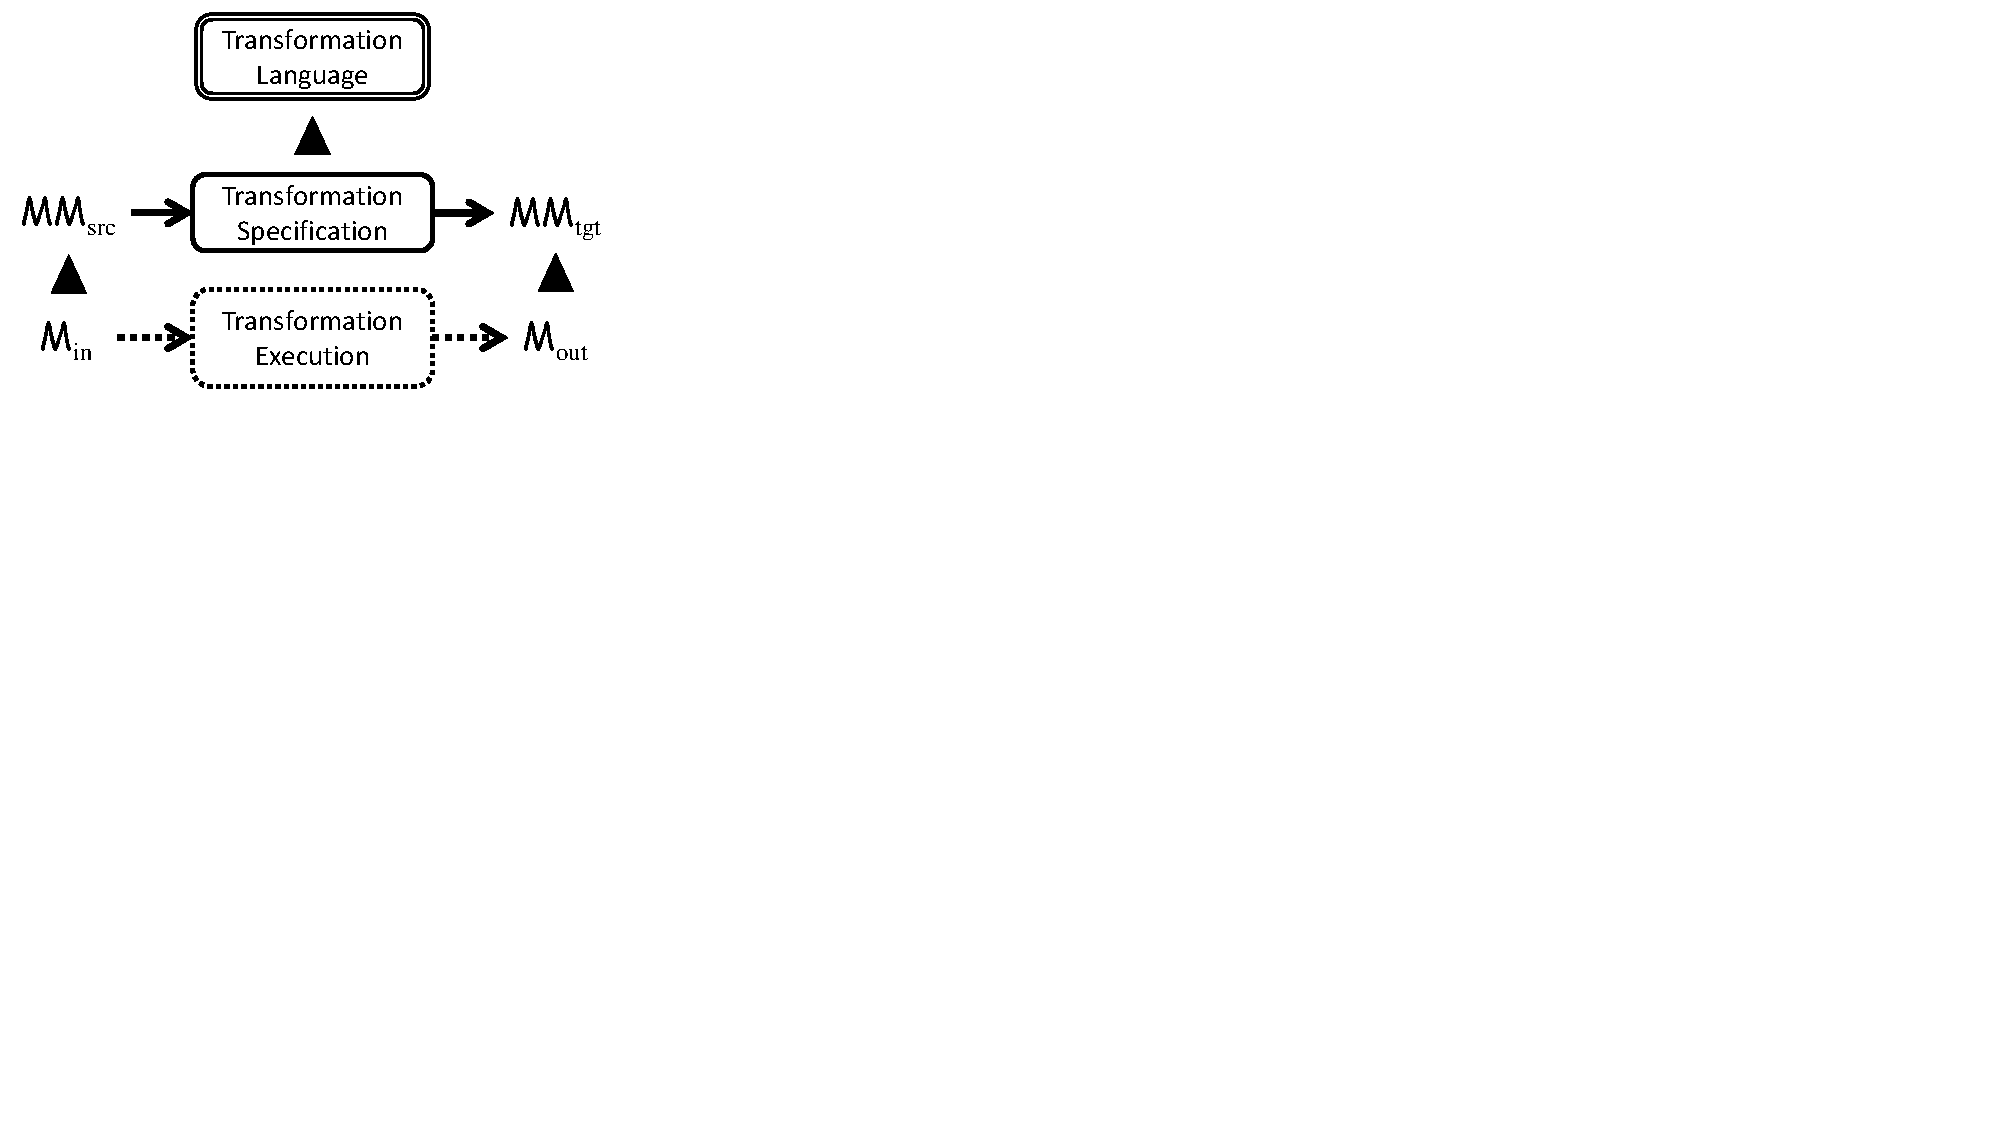
\includegraphics[width=\columnwidth,page=1,clip, trim=0.3cm 12.5cm 23.5cm 0.2cm]{ModelTransformation.pdf}
   \end{minipage}
   \hfill
   \begin{minipage}[b]{0.48\columnwidth}
   \includegraphics[width=\columnwidth,page=2,clip, trim=0.5cm 13.7cm 19.3cm 0cm]{ModelTransformation.pdf}%
   \end{minipage}
   \caption{Model \emph{Transformation} (MT) (left) and Model \emph{Animation} (MA),
   as a special case of MT, operating on the \emph{concrete syntax} of model $\mathsf{M}$,
   which is involved in an endogenous, in-place \emph{simulation} MT. Metamodels
   $\mathsf{MM}$ and $\mathsf{MM}_{\mathsf{CS}}$ may be related through rendering/parsing}%
   \label{fig:MT}%
   \Description[<short description>]{<long description>}
\end{figure}


MTs are not created equal: whereas they may seem syntactically, and sometimes 
semantically, similar, they may serve different purposes (known as MT intents
\citep{J:Lucio-Amrani-etAl:2014} in the literature) that need to be adequately
distinguished. For the purpose of this paper, three different MT intents are
interesting to precisely define, because they often raise confusion in the literature.
For an input model \textsf{M},
\begin{description}
   \item[Visualisation] is an intent characterising an outplace, heterogeneous
   MT aiming at visually \emph{representing}, or \emph{rendering}, \textsf{M} 
   through the definition of a \emph{visual} concrete syntax mainly composed of 
   graphical symbols.
   
   \item[Simulation] is an intent characterising an inplace, endogeneous MT aiming
   at defining \textsf{M}'s operational semantics, i.e. how \textsf{M} evolves 
   over time during executed.
   
   \item[Animation] is ``\emph{the visual representation of a simulation}'' 
   \citep{J:Lucio-Amrani-etAl:2014}, i.e. it visually renders the computations steps
   defined by the MT simulation specification, by visually projecting the changes
   operated on the simulated model through its (visual) concrete syntax.
\end{description}
Summarising, an \emph{animation} is tightly connected to a \emph{simulation} through
the use of a(n existing) \emph{visualisation}.
In other terms, designing an MA requires the following components, as depicted 
in \autoref{fig:MT} (right):
\begin{itemize}
	\item A Concrete Syntax \textsf{CS} that should be defined over \textsf{MM}, so
   that it becomes possible to \emph{visualise} \textsf{M} as a graphical model 
   $\mathsf{M}_{\mathsf{CS}}$.
   
   \item \textsf{MM}'s operational semantics is specified in a \emph{simulation}
   MT (specification).
   
   \item \emph{during} each run of the simulation's execution, the computing steps
   are visually rendered over $\mathsf{M}_{\mathsf{CS}}$.
\end{itemize}

Just like MTs are built over transformation \emph{units}, i.e. basic building blocks
that are composed to realise larger, complex transformations, it is likely that 
MA requires a similar decomposition process into basic ``units'' to build and 
organise them. However, MTs are likely specified independently of any MA, primarily
for capturing the \DSL's behaviour, but also likely for supporting other activities
(typically, code generation, and various analyses, among others). Since both an MT
and an MA for a given model \textsf{M} exist for different purposes, it seems 
reasonable to build them separately, and even to entrust their specification to
different persons, or teams, thus creating a new \emph{role} in \MDE: the 
\emph{MA Designer}, who need adequate methodologies and tools to perform the job.

Although serving different concerns, MT and MA are by nature tightly connected,
since they both encode a \DSL's behaviour. A Model Transformation Unit (TU) is the
smallest, coherent unit of computation visible from the outside. An interesting
approach would consist in directly relating, or connecting, the (execution of) a
Model Animation Unit (AU) to (the execution of) a TU, so that the changes performed
inside the TU are visually rendered. 

However, to fully unlock the potential of MA engineering, the specification of UAs
should be completely decoupled from the specification of (and languages for) TUs.
As they serve a common purpose, a mechanism for explicitly relating UAs to corresponding
TU(s) is required for this vision to work: when the execution engine of the MTL
executes a TU, it passes information to the MA engine to concurrently run the
animation. This vision is directly inspired by how existing methodologies for designing 
debuggers for MTLs \citep{bousse2018omniscient,J:VanMierlo-Vangheluwe-etAl:2020}:
to avoid inspecting models that may be inconsistent during the execution of a TU,
a so-called debugging \emph{step} is defined by annotating TUs relevant for inspection.
An execution \emph{step} provides the support for animation steps.

Conceptually, TUs and AUs should be in an \textsf{N:N} relationship, as depicted
in \autoref{fig:TU-AU}
\begin{itemize}
	\item A TU may be connected to several AUs, in order to provide different abstraction
   levels, and multiple views on the same execution (part). Typically, a beginner
   may need detailed visual information to understand a specific part of a model's
   execution, while a more advanced user may be happy with minimal animation.

   \item An AU may be connected to several TUs, likely integrated in simulations
   for different models. Associated with appropriate composition operators, this
   approach promotes the definition of AUs libraries that capture popular and 
   widely used animation \emph{patterns}, thus enabling modularity and reuse 
   across \DSLs.
\end{itemize}

\begin{figure}[t]%
   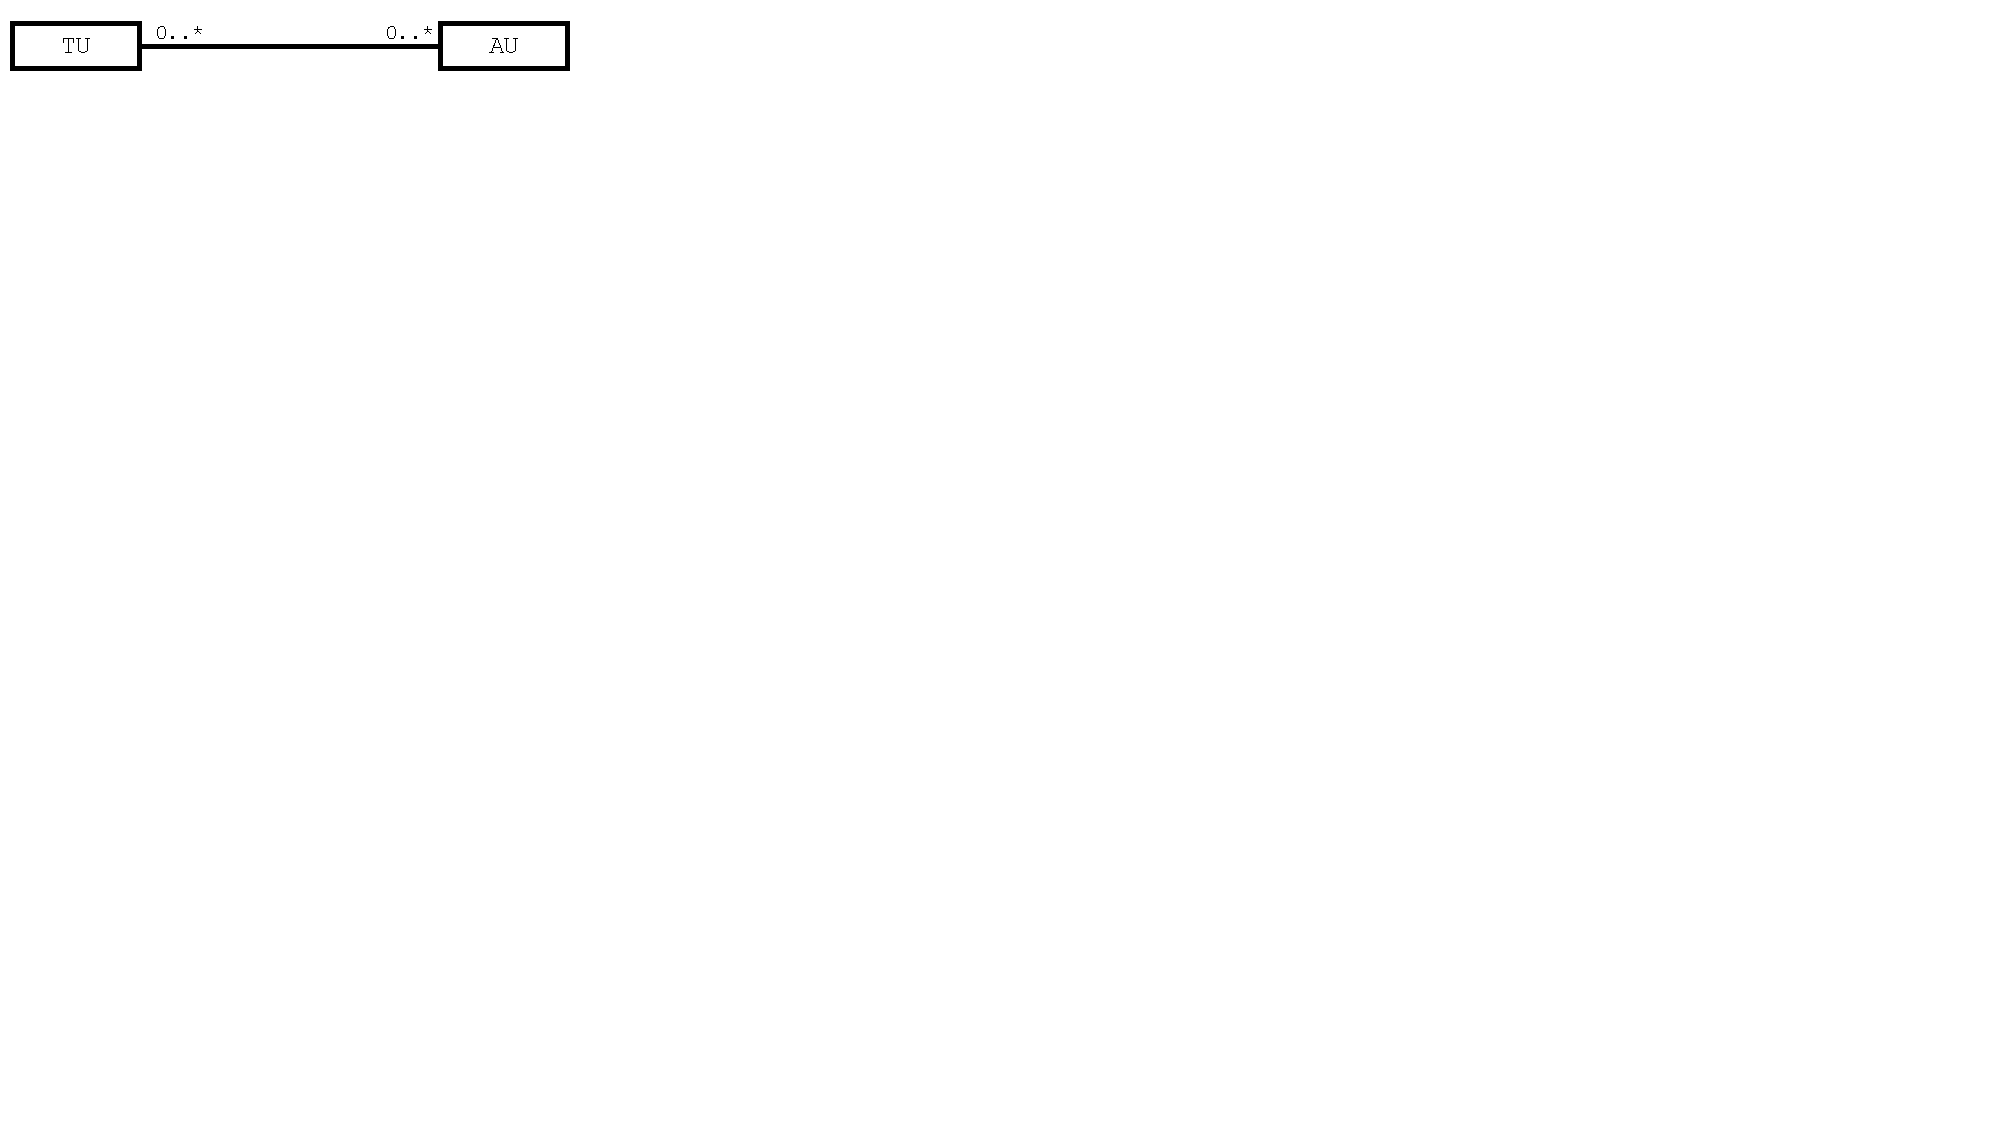
\includegraphics[width=\columnwidth,clip, trim=0cm 17.8cm 24.2cm 0.2cm]{TU-AU}%
   \caption{Relationship between Transformation (TU) and Animation (AU) Units for
   promoting multi-abstraction, and reuse.}%
   \label{fig:TU-AU}%
\end{figure}

To summarise our vision for enabling a systematic design of MA, we assume that a 
\DSL Engineer has already defined the core components, i.e. a metamodel capturing
the abstract syntax, one concrete syntax allowing to create, edit and manage 
conforming models, and a simulation that captures the \DSL's behaviour, specified
in an MTL that defines identifiable TUs. The missing steps, and corresponding challenges,
for an MA Engineer, would be the following:

\begin{description}
   \item[C1.] How to explicitly model a Concrete Syntax, with sufficient details
   to support animation? Since MA basically consists of continuously updating the
   concrete syntax of a \DSL along its execution, an explicit representation of the
   concrete syntax that exposes the graphical features to the MA designer is 
   required.
   
   \item[C2.] How to explicitly model an MA compositionally, i.e. by creating an
   MA using basic components that are progressively composed in a fully-fledged
   animation representing the \DSL's behaviour visually? 
   
   \item[C3.] How to explicitly map TUs describing a \DSL's behaviour with the
   appropriate AU(s)? 
\end{description}

\section{DSL Examples}
\label{sec:Examples}

We now present three simple \DSMLs, namely \textsf{PacMan}, Finite State
Machines (\textsf{FSM}), and Petri Nets (\textsf{PN}), following the same 
outline:
\begin{itemize}
	\item The \DSL's structure is specified using a metamodel expressed in \MOF;
   we also informally specify a possible \emph{concrete syntax}, then provide a 
   simple witness model.

   \item The \DSL's semantics is sketched, without details of implementations that
   highly depend on (i) the MTL used, and (ii) the modelling style of the MT designer. 
   We however show how possible implementations in different MTLs, for \textsf{PacMan},
   may lead to a similar MT structure (and TUs supporting animation), 
   in a way that is agnostic of the underlying MTL.

   \item A family of animations are then described in detail, and numbered for 
   future reference.
\end{itemize}
Note that we assume that the \DSL structure follows the Executable \DSML Pattern
\citep{Combemale-Cregut-Pantel:2012}, which consists of two separate metamodels for
defining executable \DSMLs:
\begin{itemize}
	\item The so-called \emph{Domain Definition} metamodel captures the 
   \emph{static} structure of the \DSL, which typically serves for defining valid
   models using various textual and/or visual syntaxes;
   
   \item The \emph{State Definition} metamodel adds new information on top of the
   Domain Definition metamodel to enable state-based execution, thus defining those
   elements that are modified during execution.
\end{itemize}
Both metamodels typically need to be merged, using different techniques (e.g.,
using \MOF's ``package merge'' approach \cite{TR:OMG-MOF:2016}, or other 
composition techniques \cite{J:Abouzahra-Sabraoui-Afdel:2020}).
For clarity and presentation simplification purposes, we depicts both metamodels
in a merged fashion, although we visually distinguish each part: the Domain Definition
metamodel elements are represented using the regular font with plain arrows for MOF 
references; while the State Definition elements use curvy fonts and dotted MOF references.

\subsection{\textsf{PacMan}: A \DSL for the PacMan game}
\label{sec:Examples:PacMan}

The PacMan game is a popular arcade game that gained interest in the \MDE community
because it captures a well-known, simple reactive \DSL with an easily understandable
concrete syntax, and presents interesting real-time features for execution. 

\subsubsection{Specification}
\label{sec:Examples:PacMan:Specification}

On the top left compartment is represented a metamodel
$\mathsf{MM}_{\mathsf{PM}}$, as created by a DSL engineer. A \textsf{Game} 
consists of a sequence of \textsf{Level}s, each displaying a \textsf{Maze} where
\textsf{Persona}s evolve. A \textsf{Level} terminates when \textsf{PacMan} is eaten
by a \textsf{Ghost}, or when it has eaten all \textsf{Cookie}s. Several players
may compete for the highest \textsf{Score}.

On the top right compartment, a basic model $\mathsf{M}_{\mathsf{2x2}}$ with a
\textsf{unique} \textsf{Level} of size 2x2, as possibly created by a modeller,
is depicted using three different concrete syntaxes:
textual for $^{\mathsf{TXT}}\mathsf{M}_{\mathsf{2x2}}$ (inspired by eMotions 
\cite{J:RiveraDuranVallecillo:2009}); based on UML Object Diagram for
\cite{B:Rumbaugh-Jacobson-Booch:2004} for $^{\mathsf{OD}}\mathsf{M}_{\mathsf{2x2}}$;
and freely inspired by the real game for $^{\mathsf{Viz}}\mathsf{M}_{\mathsf{2x2}}$,
the two latters being graphical.

\begin{figure*}[t]
   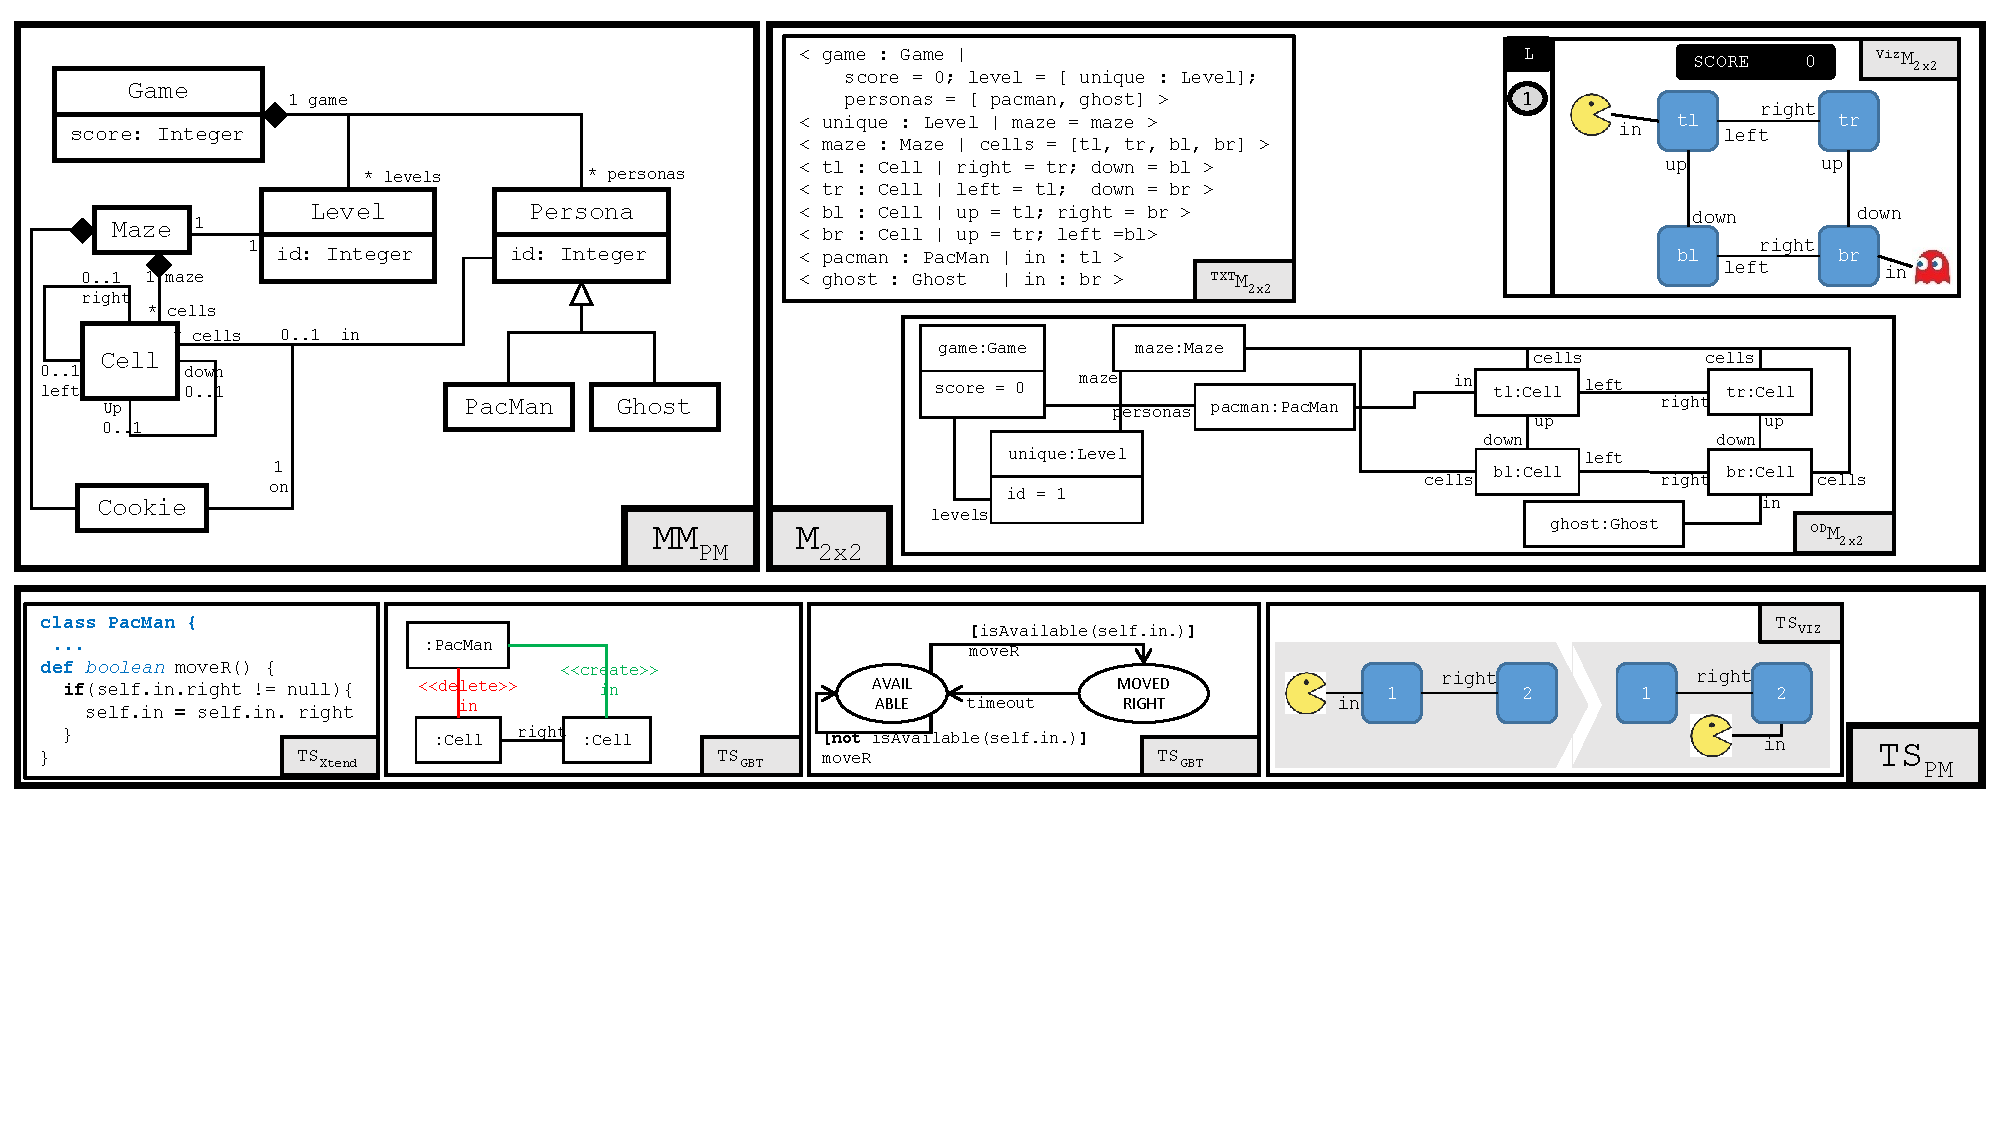
\includegraphics[width=\textwidth,clip, trim=0cm 5.5cm 0cm 0cm]{MM-M-T.pdf}
   \caption{Specifying a Pac-Man DSL: the DSL engineer create the metamodel 
   $\mathsf{MM}_{\mathsf{PM}}$; a modeller chooses a concrete syntax to create
   a simple model $\mathsf{M}_{\mathsf{2x2}}$; a MT designer specifies a transformation
   $\mathsf{TS}_{\mathsf{PM}}$ (only the \emph{\textsf{moveR}} MT unit is shown)}
   \label{fig:PacMan}
   \Description[<short description>]{<long description>}
\end{figure*}

\subsubsection{Execution}
\label{sec:Examples:PacMan:Execution}

The bottom compartment of \autoref{fig:PacMan} describes a simple rule 
\emph{\textsf{moveR}} (moving Pac-Man on a \textsf{Cell} at its right, if 
available) as part of the simulation MT specification $\mathsf{TS}_{\mathsf{PM}}$,
as part of $\mathsf{MM}_{\mathsf{PM}}$'s executable semantics. 
The first MT, $\mathsf{TS}_{\mathsf{Xtend}}$, uses metaprogramming 
(based on Xtend with GeMoC \cite{Leroy-Bousse-etAl:2017}). The next and last ones
are based on Graph Transformations: $\mathsf{TS}_{\mathsf{GBT}}$ relies on 
$^{\mathsf{OD}}\mathsf{M}_{\mathsf{2x2}}$ to express the rewriting (as would be 
expressed e.g. in Henshin \cite{Bill-Gabmeyer-Kaufmann-Seidl:2014}); 
while $\mathsf{TS}_{\mathsf{VIZ}}$ relies on $^{\mathsf{Viz}}\mathsf{M}_{\mathsf{2x2}}$
(as would be expressed e.g. in AtoMPM \cite{J:SyrianiVangheluwe:2013}). 
Finally, $\mathsf{TS}_{\mathsf{FSM}}$ presents an MT fragment expressed with 
a UML's Finite State Machine \cite{B:Rumbaugh-Jacobson-Booch:2004}. 
Note that all MT specifications (fragments) but $\mathsf{TS}_{\mathsf{Xtend}}$ 
present a graphical representation, showing that MT specifications may well be 
graphically visualised as well.

\subsubsection{Animations}
\label{sec:Examples:PacMan:Animations}

The PacMan game typically uses three kinds of animations for different situations:
\begin{description}
   \item[A \textsf{Persona} moves.] Typically, a specific animation could be attached
   to each movement, as they are traditionally encoded in different rules/operations
   (cf. e.g. \textsl{moveR} as specified in \autoref{fig:PacMan}, but also 
   \textsl{moveL}, \textsl{moveU} and \textsl{moveD} for moving left, up and down).
   Depending on whether the MTL allows using abstract classes (which would be 
   \textsf{Persona} here) for MT specification, these rules/operations may need 
   to be duplicated. 
   
   \item[\textsf{PacMan} eats a \textsf{Cookie}.] This occurs when \textsf{PacMan} is on a \textsf{Cell}
   that contains a \textsf{Cookie}, making it disappear and triggering a 
   \textsf{Score} update.
   
   \item[\textsf{PacMan} is eaten by a \textsf{Ghost}.] This occurs when 
   \textsf{PacMan} is on the same \textsf{Cell} as a \textsf{Ghost}, which may occur
   by either \textsf{Persona} making a move to an already occupied \textsf{Cell}.
\end{description}
To summarise, we would have to define four different animations to fully animate
the \textsf{PacMan} \DSL:
\begin{description}
   \item[PM.1] The \textsf{Persona} disappears from one \textsf{Cell} and reappears
   on another (adjacent) \textsf{Cell}.
   
   \item[PM.2] Assuming \textsf{PacMan} is on a \textsf{Cell} containing a \textsf{Cookie},
   the \textsf{Cookie} disappears.
   
   \item[PM.3] The \textsf{Score} is updated by a given increment. 

   \item[PM.4] Assuming \textsf{PacMan} and a \textsf{Ghost} are on the same
   \textsf{Cell}, \textsf{PacMan} disappears.
\end{description}
Note that those animations are not completely unrelated. First, \textbf{PM.2} and
\textbf{PM.3} need to be conducted sequentially quickly enough to not notice a
time gap. Second, \textbf{PM.2} and \textbf{PM.4} appear to be very similar in
nature: they both assume that two objects are located on the same \textsf{Cell} 
before making one of them disappear.

\subsection{\textsf{FSM}: A \DSL for Finite-State Machines}
\label{sec:Examples:FSM}

Finite State Machines (FSM) represent a common \DSL for capturing state-based 
behaviour of various biological, but also computational domains (e.g. Turing 
Machines, but also Chomsky's Regular Grammars, among others). This Section considers
FSMs that are simplified in various ways: in particular, we only consider a
word acceptance semantics where transitions do not contain guards and triggers are
reduced to their simplest expression, namely simple strings.

\subsubsection{Specification}
\label{sec:Examples:FSM:Specification}

\begin{figure}%
   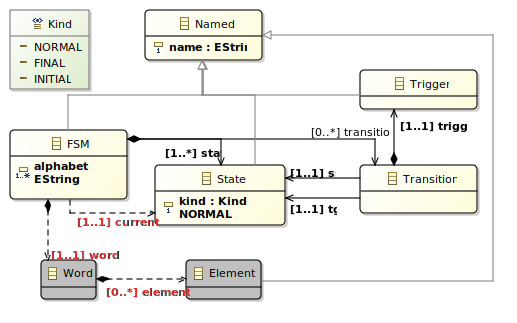
\includegraphics[width=\columnwidth]{FSM}%
   \caption{A metamodel for Finite State Machines.}%
   \label{fig:FSM_MM}%
\end{figure}


\autoref{fig:FSM_MM} (top) specifies the metamodel of the Finite State Machine \DSL. 
An \textsf{FSM} is composed of \textsf{State}s identified by a \textsf{name}, and
\textsf{Transition}s that contain a simple \textsf{Trigger}, specified as 
\textsf{name}d event. \autoref{fig:FSM_M} depicts a simple model consisting of 
three \textsf{State}s and three \textsf{Transition}s, to recognise the regular 
expression $\mathtt{(a\cdot b)^\star\ b}$. 

We assume the classical visual representation for \textsf{FSM}: a \textsf{State}
is represented by a circle labelled with its \textsf{name}; and a 
\textsf{Transition} is represented by an arrow pointing to its \textsf{tgt} and 
carrying the \textsf{Trigger}'s name as a label. We represent the \textsf{current}
\textsf{State} by surimposing a red rounded form (that we call \emph{token}) over
the corresponding \textsf{State} (cf. \autoref{fig:FSM_M}).


\subsubsection{Execution}
\label{sec:Examples:FSM:Execution}

We adopt a \emph{word-recognising} semantics encoded in a transformation called
\textsf{accept} that reads a \textsf{Word} and traverses the \textsf{FSM}. A 
\textsf{Word} is accepted iff the \textsf{current} \textsf{State} of the \textsf{FSM}
is \textsf{FINAL} when the \textsf{Word} becomes empty.

\subsubsection{Animations}
\label{sec:Examples:FSM:Animations}

Typically, \textsf{accept} is implemented using a sub-transformation 
\textsf{fire(e : Element) : State [0..1]} that determines which \textsf{State} 
to update to when consuming an \textsf{Element} \textsf{e}, making it a good 
candidate for four different animations, when \textsf{fire} returns an actual 
\textsf{State}:
\begin{description}
   \item[FSM.1] The token disappears from the \textsf{current} \textsf{State} and
   reappears inside the updated \textsf{current};
   \item[FSM.2] The token disappears from the \textsf{current} \textsf{State}, and
   slides along the entire arrow of the fired \textsf{Transition}, then appears in
   the updated \textsf{current};
   \item[FSM.3] The token disappears from the \textsf{current} \textsf{State}, the
   arrow of the fired \textsf{Transition} blinks in red for 2 seconds, then the 
   token reappears in the updated \textsf{current}.
\end{description}


\begin{figure}[t]%
   \centering
   \begin{subfigure}[b]{0.45\columnwidth}
      \centering
      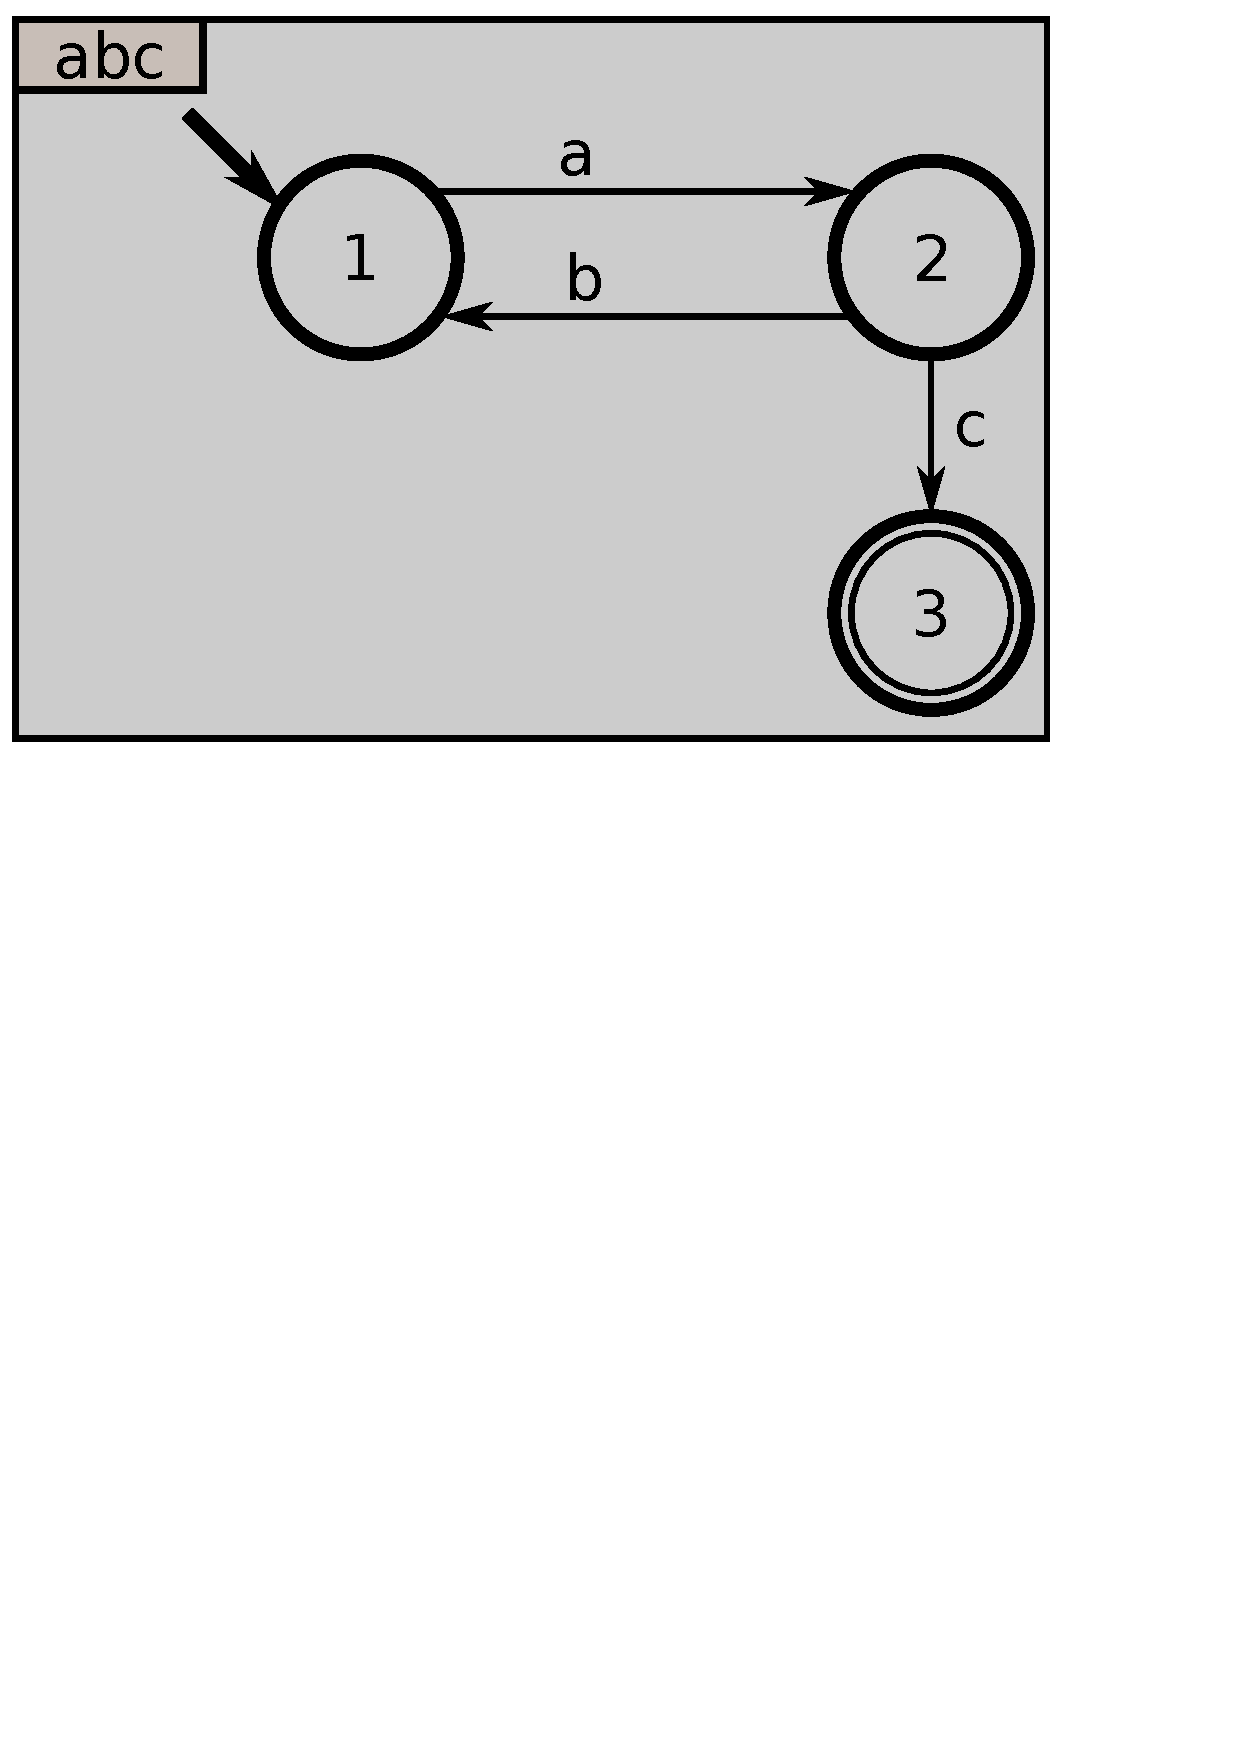
\includegraphics[width=\columnwidth, clip, trim=0cm 17cm 3cm 0cm]{FSM_M.pdf}%
      \caption{Editing \textsf{abc} to obtain a 3-state/3-transition FSM model: 
      states \textsf{1} and \textsf{3} are respectively \textsf{INITIAL} and 
      \textsf{FINAL}.}
      \label{fig:FSM:Model:Edition}
   \end{subfigure}
   \hfill
   \begin{subfigure}[b]{0.45\columnwidth}
      \centering
      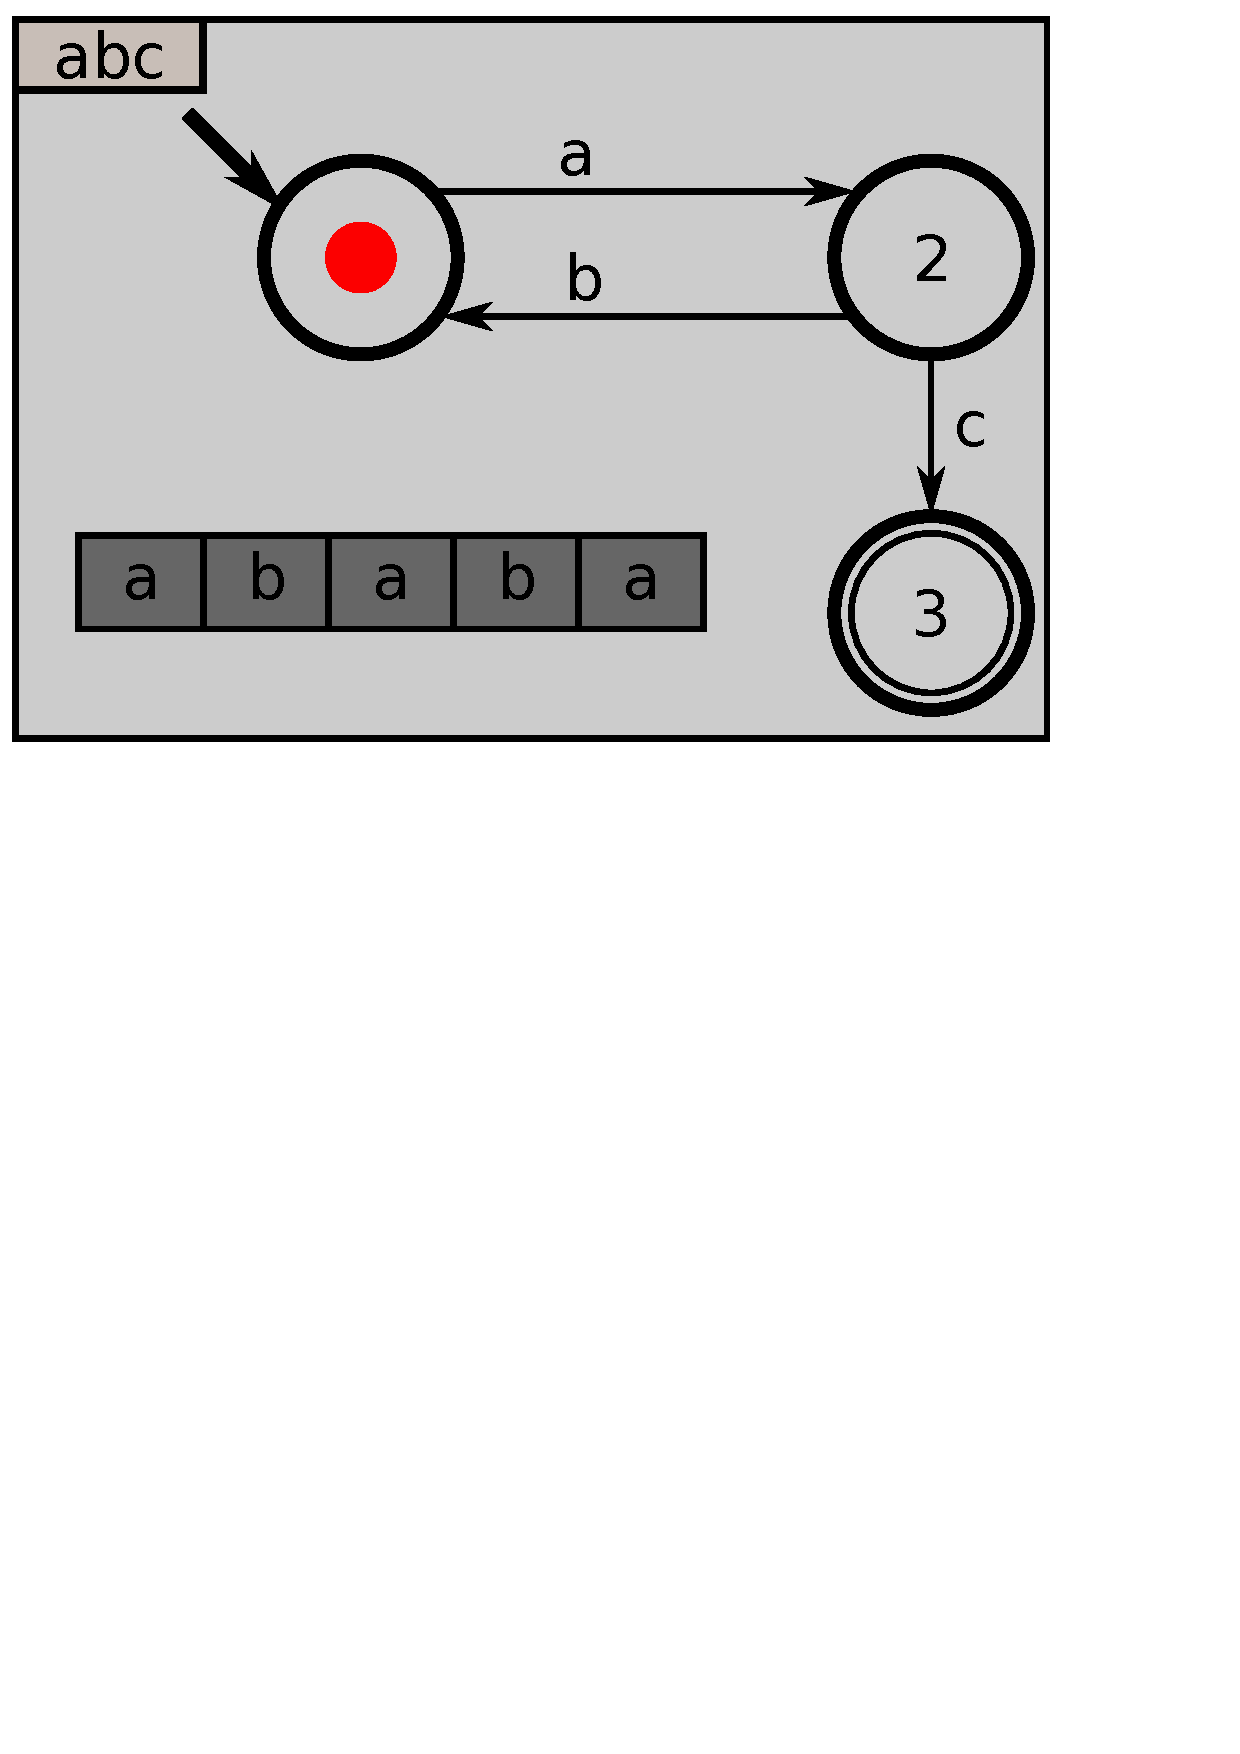
\includegraphics[width=\columnwidth, clip, trim=0cm 17cm 3cm 0cm]{FSM_MX.pdf}%
      \caption{Starting executing \textsf{abc}: the \textsf{current} 
      \textsf{State} is overlayed with a red token, and attempting to accept the
      word \textsf{ababa}.}
      \label{fig:FSM:Model:Execution}
   \end{subfigure}
  
   \vskip\baselineskip
   \begin{subfigure}[b]{0.45\columnwidth}
      \centering
      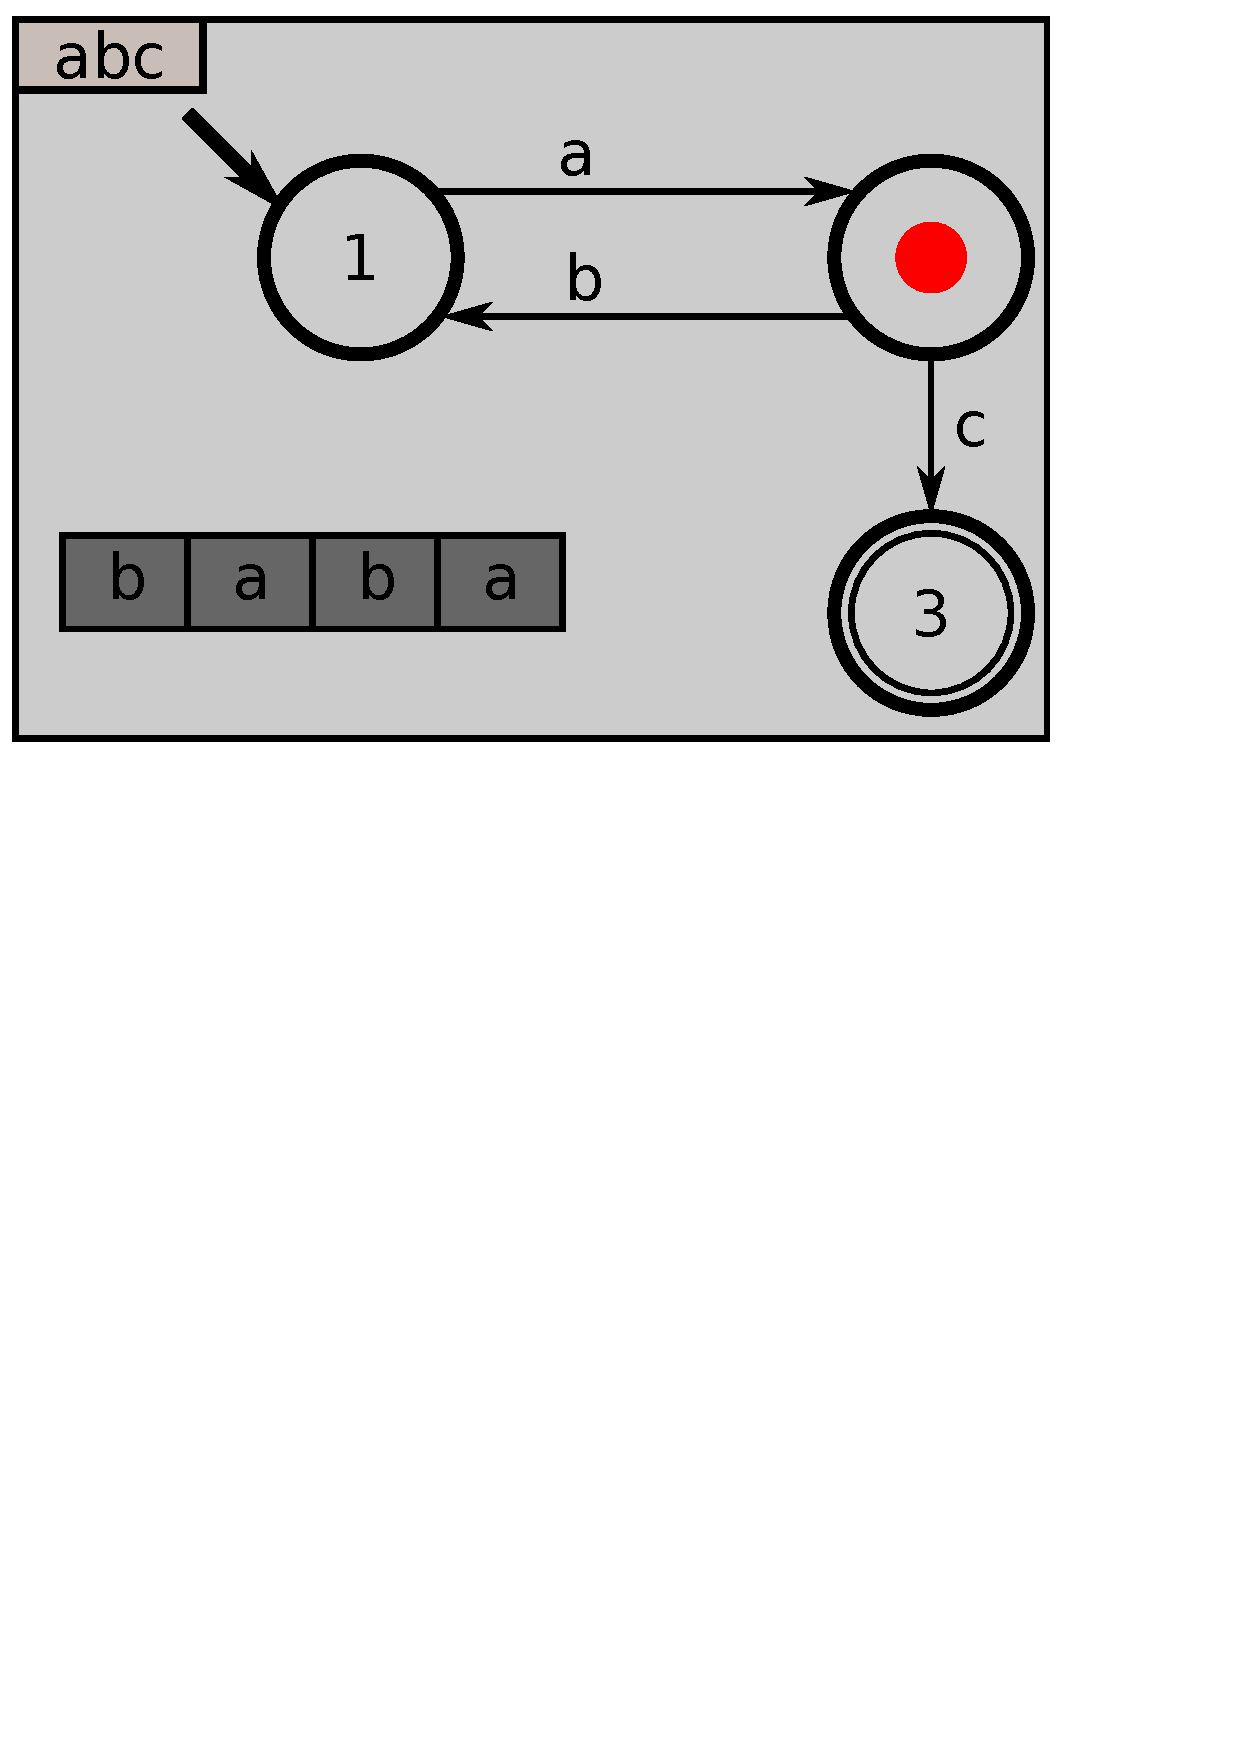
\includegraphics[width=\columnwidth, clip, trim=0cm 17cm 3cm 0cm]{FSM_MA11.pdf}%
      \caption{\textbf{Animation FSM.1:} The first execution step moves the token in
      \textsf{State} 2 (while consuming the first \textsf{Element} \textsf{a}).}
      \label{fig:FSM:Model:Animation:FSA1.1}
   \end{subfigure}
   \hfill
   \begin{subfigure}[b]{0.45\columnwidth}
      \centering
      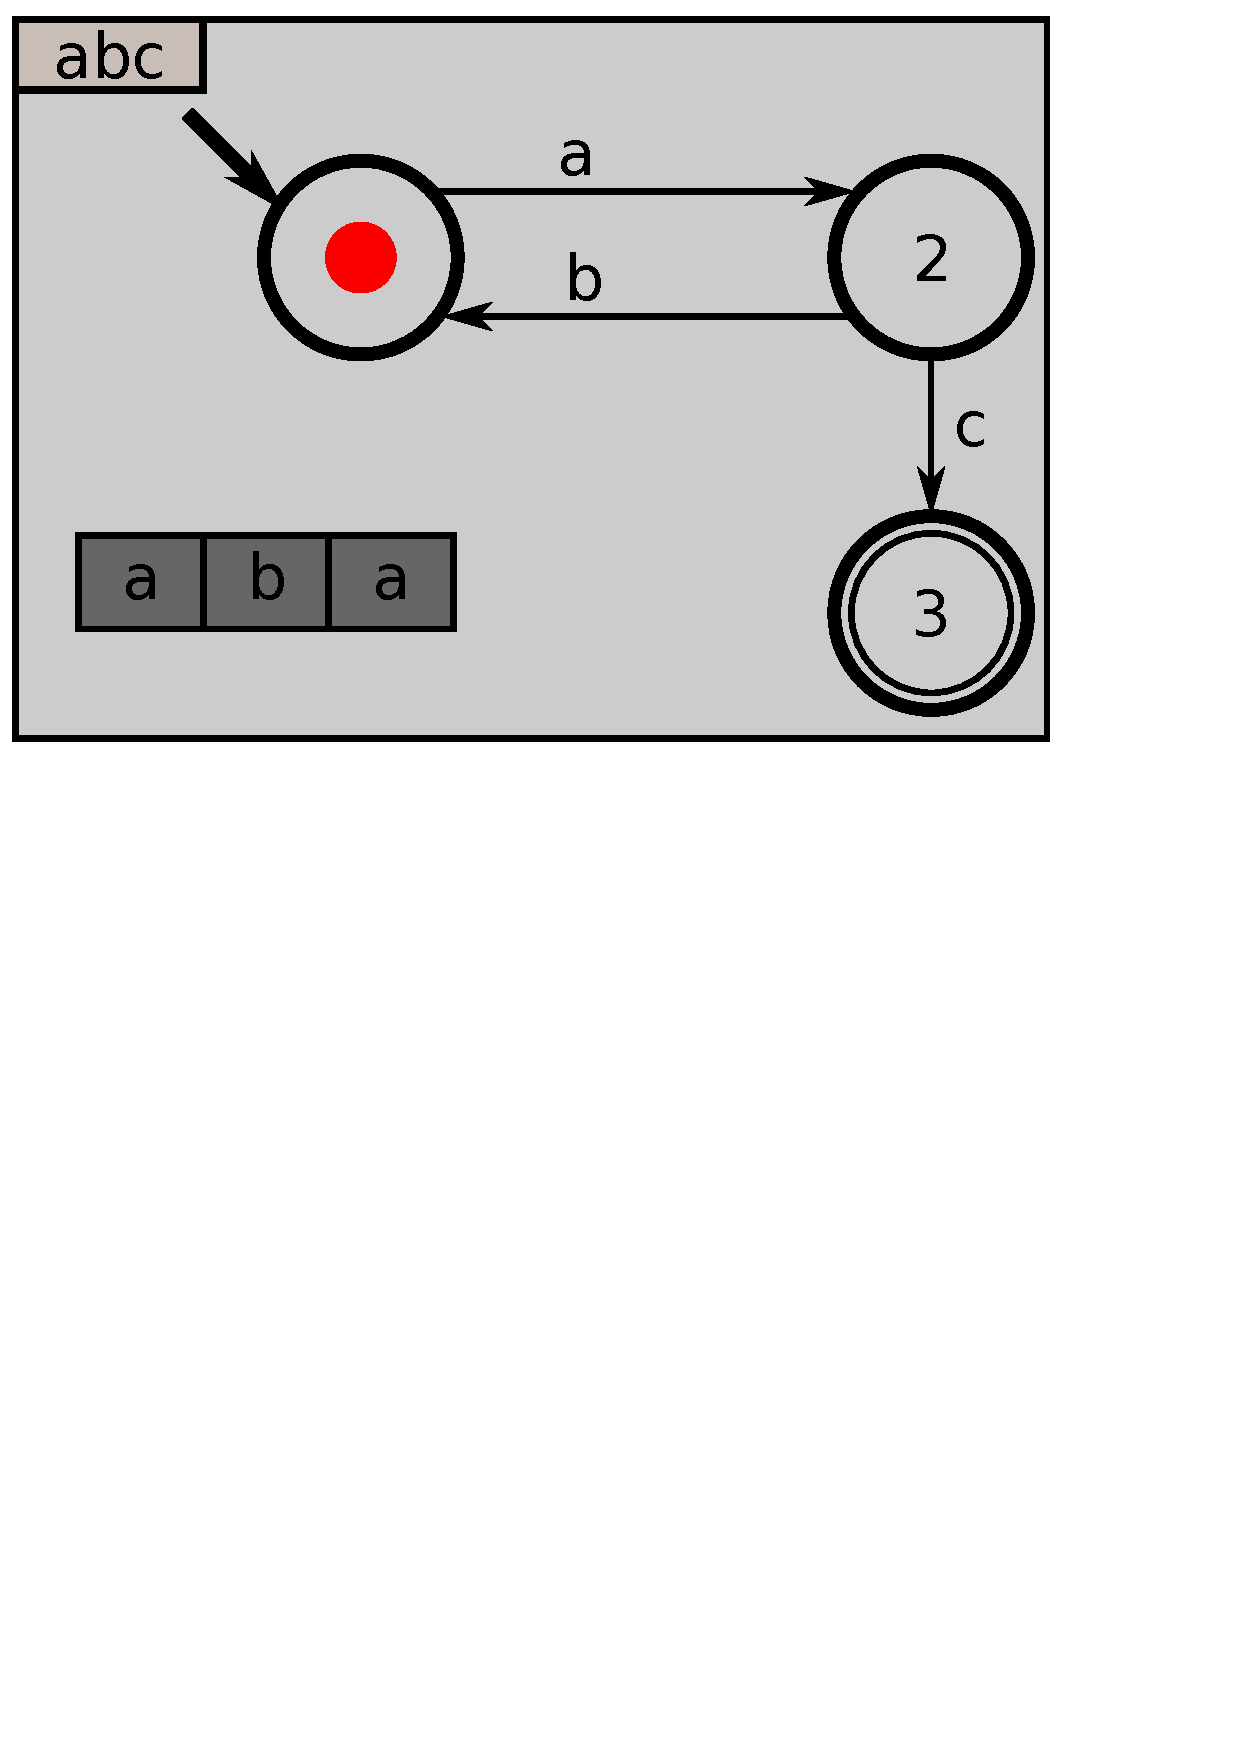
\includegraphics[width=\columnwidth, clip, trim=0cm 17cm 3cm 0cm]{FSM_MA12.pdf}%
      \caption{\textbf{Animation FSM.1:} The second execution step moves the token 
      back in \textsf{State} 1 (while consuming \textsf{b}).}
      \label{fig:FSM:Model:Animation:FSA1.2}
    \end{subfigure}
 
    \vskip\baselineskip
    \begin{subfigure}[t]{0.45\columnwidth}
      \centering
      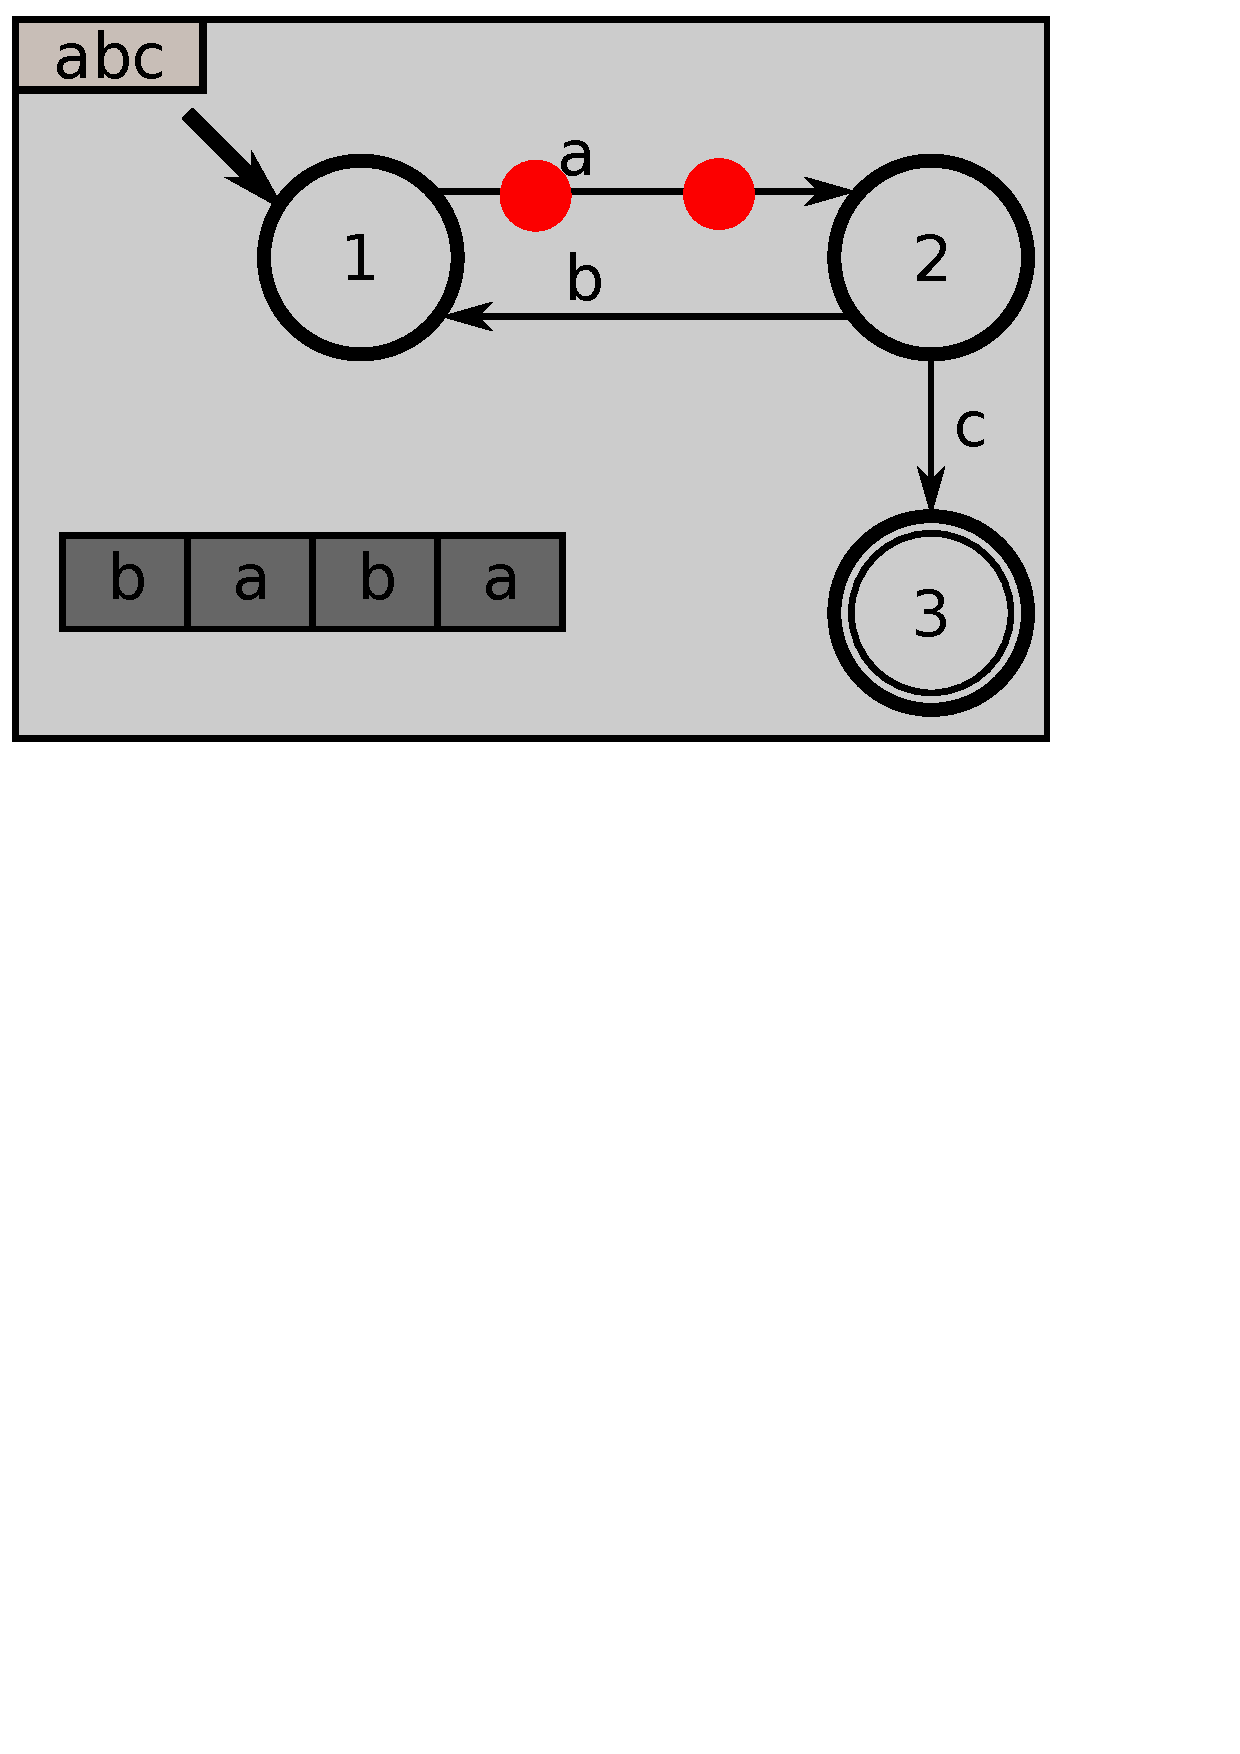
\includegraphics[width=\columnwidth, clip, trim=0cm 17cm 3cm 0cm]{FSM_MA21.pdf}%
      \caption{\textbf{Animation FSM.2:} The first phase of the animation slides
      token along the \textsf{Transition} \textsf{a} (represented here in two 
      different positions to reproduce the animation's visual effect).}
      \label{fig:FSM:Model:Animation:FSA2.1}
    \end{subfigure}
    \hfill
    \begin{subfigure}[t]{0.45\columnwidth}
      \centering
      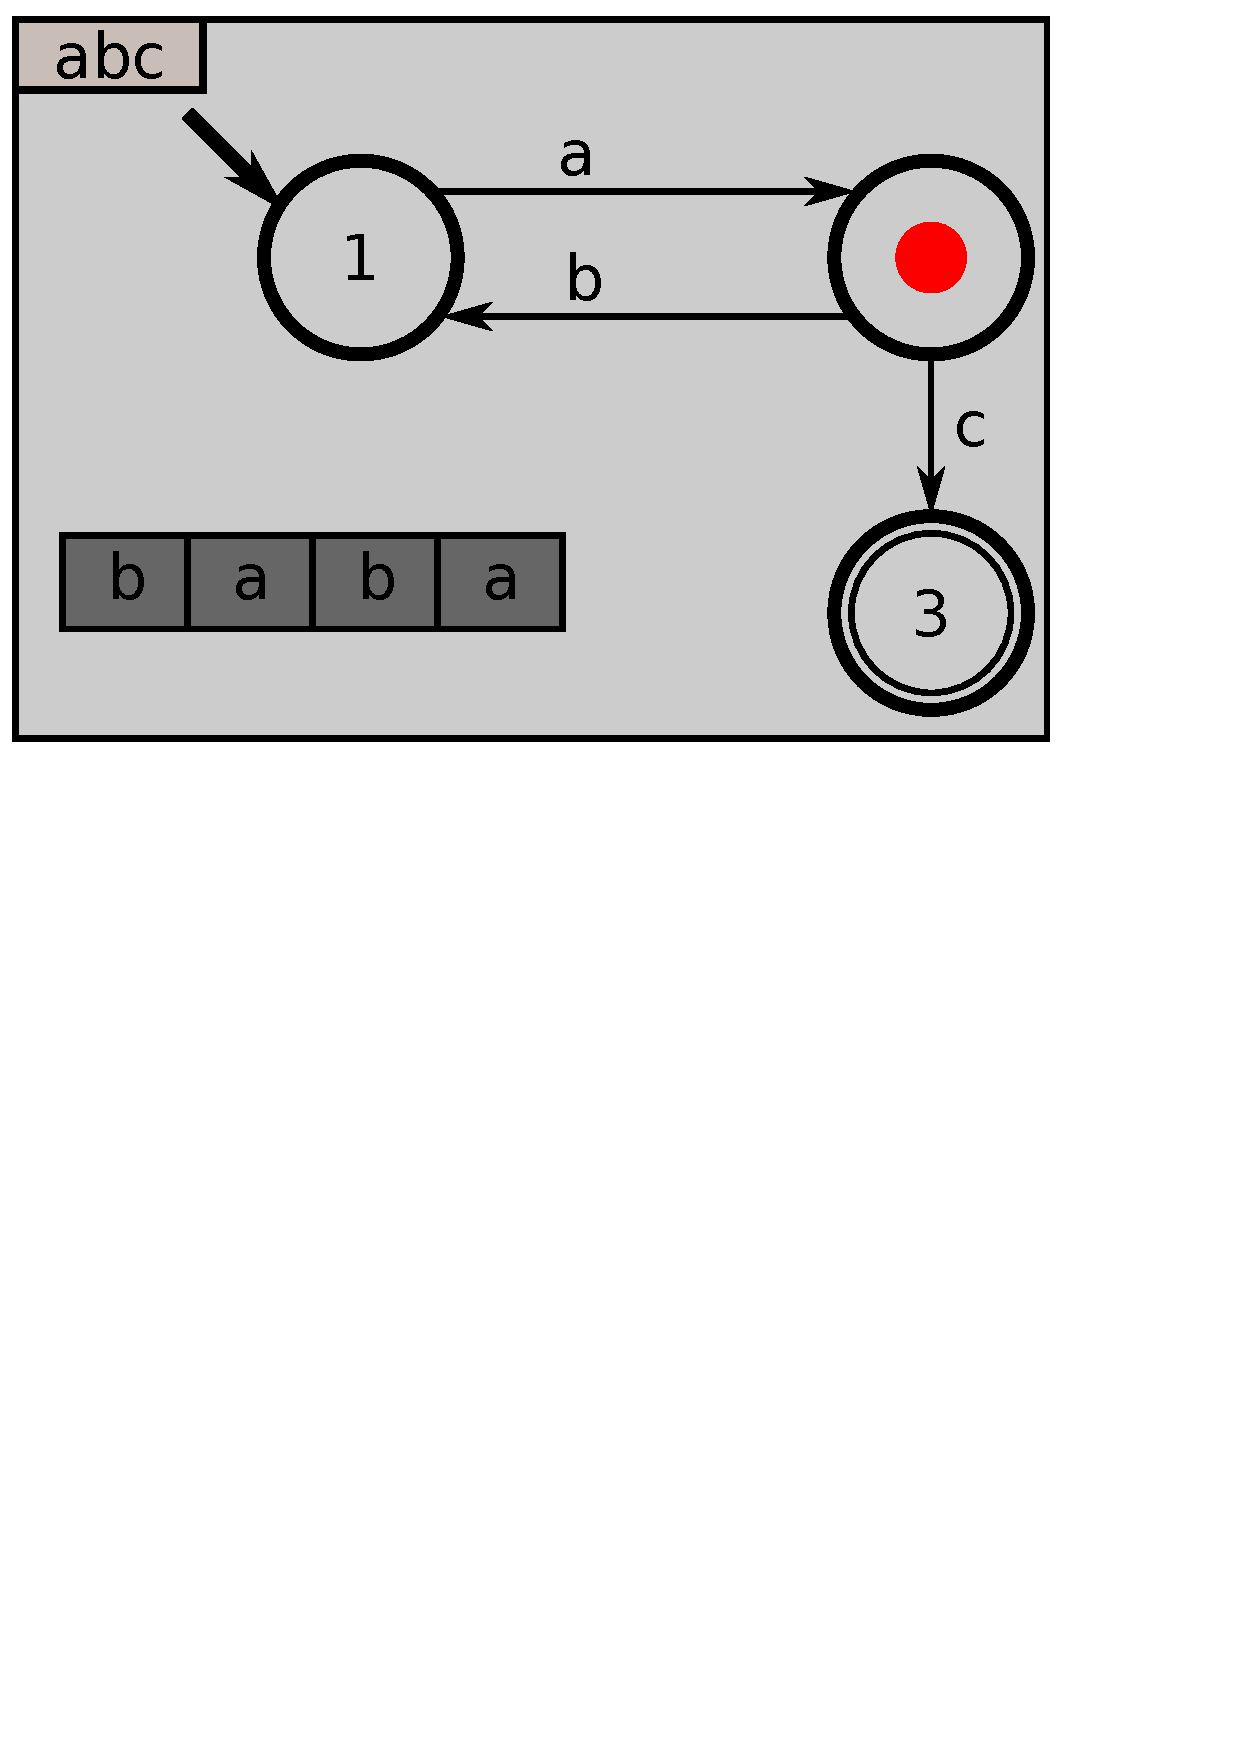
\includegraphics[width=\columnwidth, clip, trim=0cm 17cm 3cm 0cm]{FSM_MA22.pdf}%
      \caption{\textbf{Animation FSM.2:} The second phase of the animation makes
      the token appears in \textsf{State} 2, after consuming \textsf{b}.}
      \label{fig:FSM:Model:Animation:FSA2.2}
    \end{subfigure}

    \vskip\baselineskip
    \begin{subfigure}[t]{0.45\columnwidth}
      \centering
      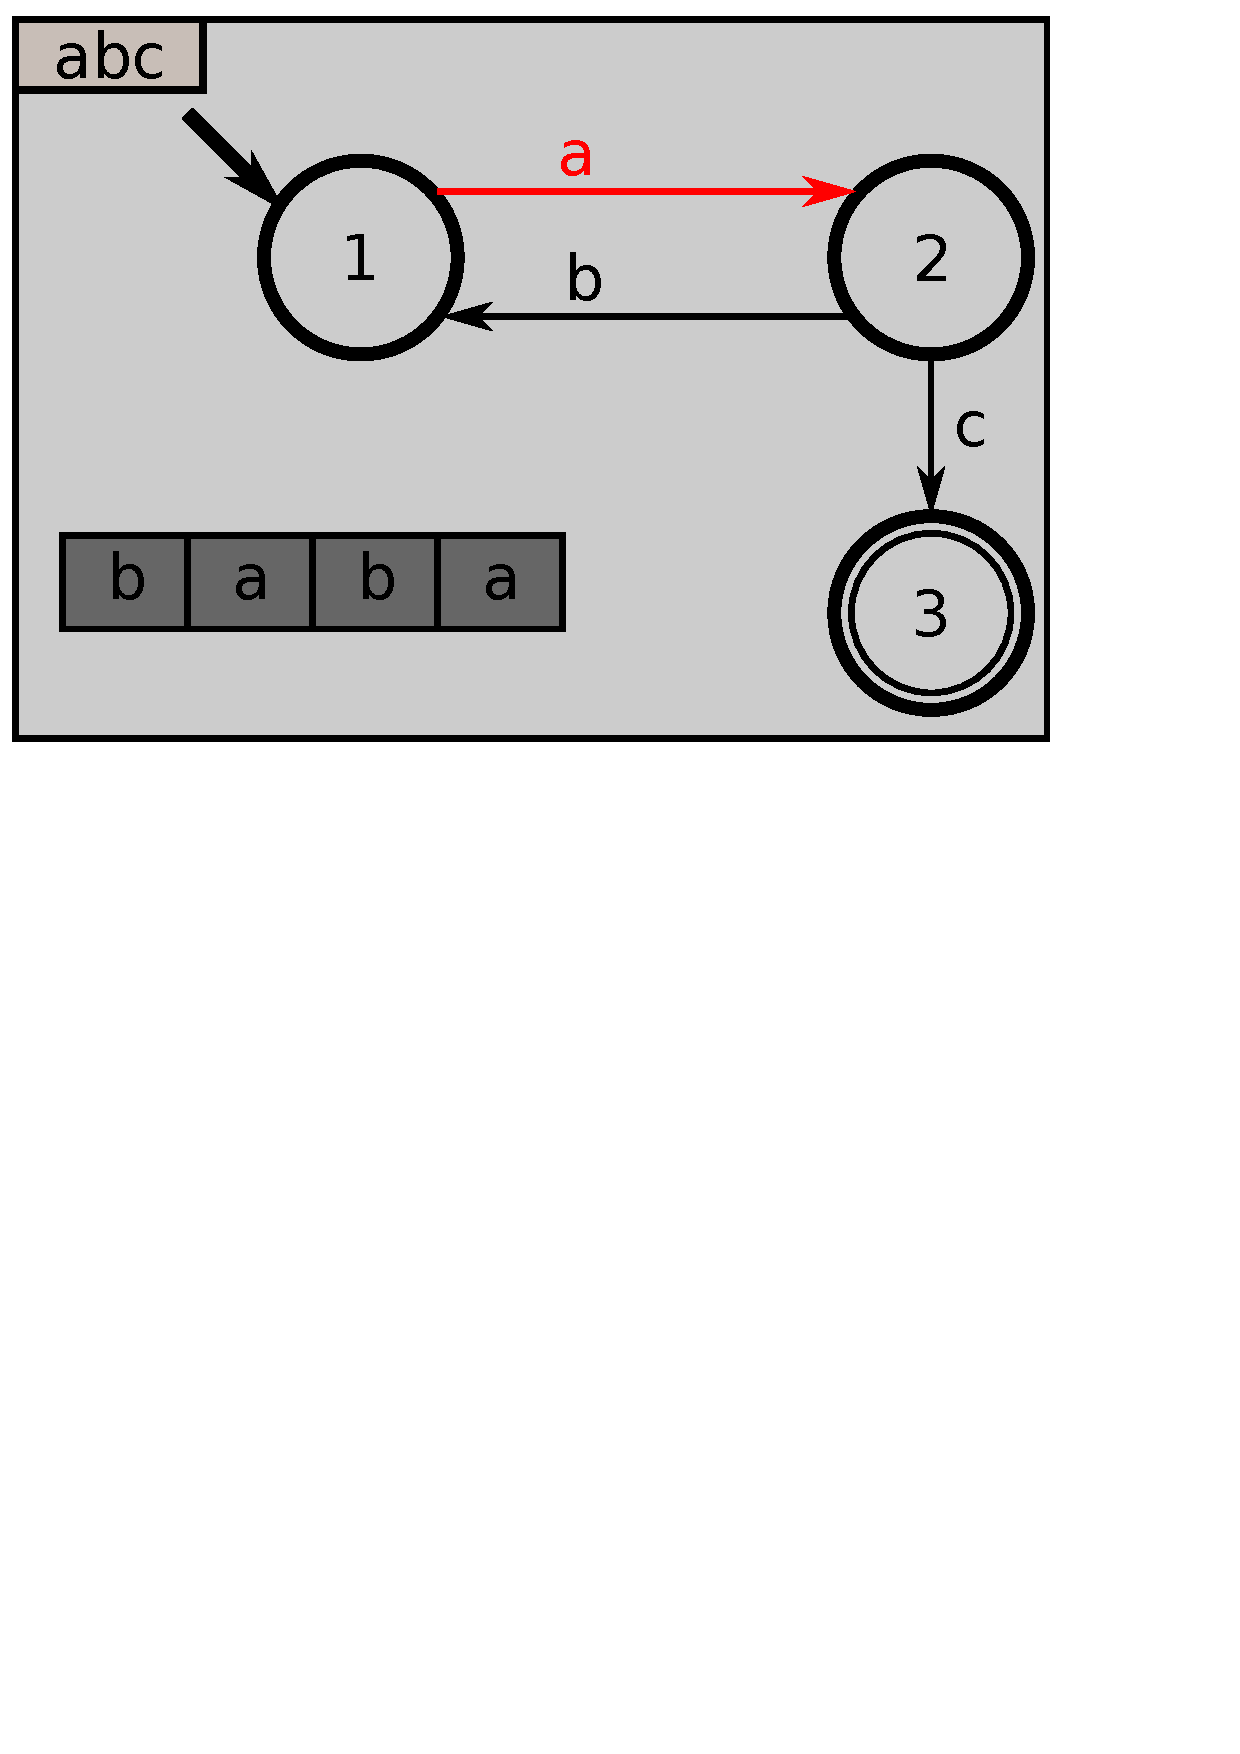
\includegraphics[width=\columnwidth, clip, trim=0cm 17cm 3cm 0cm]{FSM_MA31.pdf}%
      \caption{\textbf{Animation FSM.3:} The first phase of the animation highlights
      \textsf{Transition} \textsf{a} in red (as well as its \textsf{Trigger}).}
      \label{fig:FSM:Model:Animation:FSA2.3}
    \end{subfigure}
    \hfill
    \begin{subfigure}[t]{0.45\columnwidth}
      \centering
      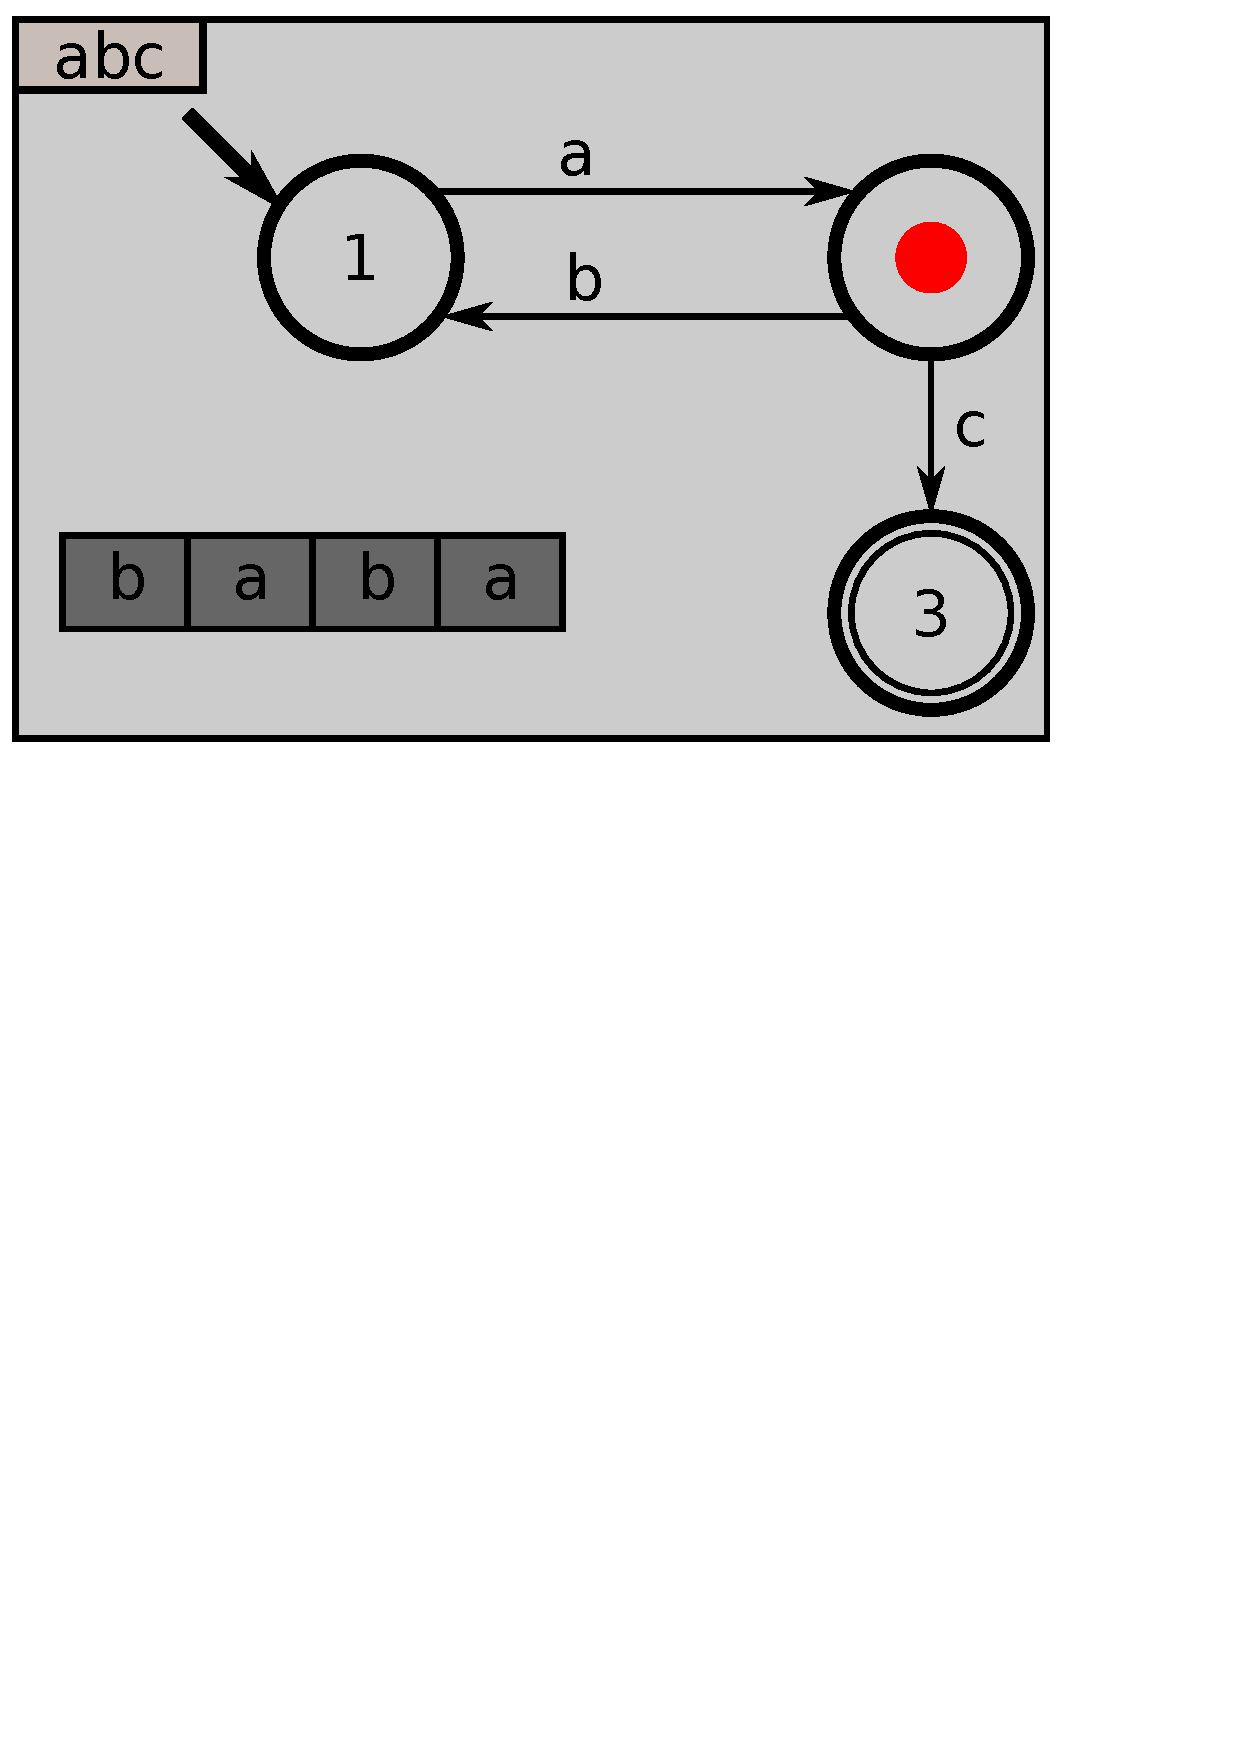
\includegraphics[width=\columnwidth, clip, trim=0cm 17cm 3cm 0cm]{FSM_MA22.pdf}%
      \caption{\textbf{Animation FSM.3:} The second phase of the animation makes
      the token appears in \textsf{State} 2, after consuming \textsf{b}.}
      \label{fig:FSM:Model:Animation:FSA2.4}
    \end{subfigure}

  \caption{\textsf{abc}: a simple model of an FSM conforming to the specification
   in \autoref{fig:FSM_MM}, and some associated animations for its execution 
   (cf. \S \ref{sec:Examples:FSM:Animations} for their specification.)}%
   \label{fig:FSM_M}%
\end{figure}


\subsection{\textsf{PN}: A \DSL for (Simple) Petri Nets}
\label{sec:Examples:PN}

\subsubsection{Specification}
\label{sec:Examples:PN:Specification}

\subsubsection{Execution}
\label{sec:Examples:PN:Execution}

\subsubsection{Animations}
\label{sec:Examples:PN:Animations}






\section{Challenges}
\label{sec:Challenges}

We now revisit the Challenges formulated at the end of \S \ref{sec:Motivation}, 
to identify key ingredients and to provide general guidelines for building 
model animators that would allow flexibility and reuse.

\subsection{Concrete Syntax (CS)}
\label{sec:CS}

The first challenge, Concrete Syntax (CS), is related to a \DSML's metamodel 
\textsf{MM} through two transformations:

$$ \mathsf{MM} \xrightleftharpoons[\mathrm{parsing}\phantom{MM}]{\phantom{MM}\mathrm{rendering}} \mathsf{CS}$$

In syntax-directed editing, \emph{parsing} is not necessary because models
are created by relying on the syntax, thus preventing ill-models. On the other hand,
\emph{rendering} is crucial for representing a model when appropriate, but
it also represents the anchor for animation. 


Having explicit MTs between \textsf{MM} and \textsf{CS} assumes indeed that 
\textsf{CS} is explicitly metamodelled: following the \MDE methodology, such
a \DSL should cover the definition of visual representations (geometric shapes as
well as various data structure representations such as tables, graphs, etc.),
but also the ability to define the rendering relationship, i.e. patterns associating
\textsf{MM}'s metamodel elements with \textsf{CS}'s elements.
We identified at least four challenges:

\begin{figure}[t]%
   \centering
   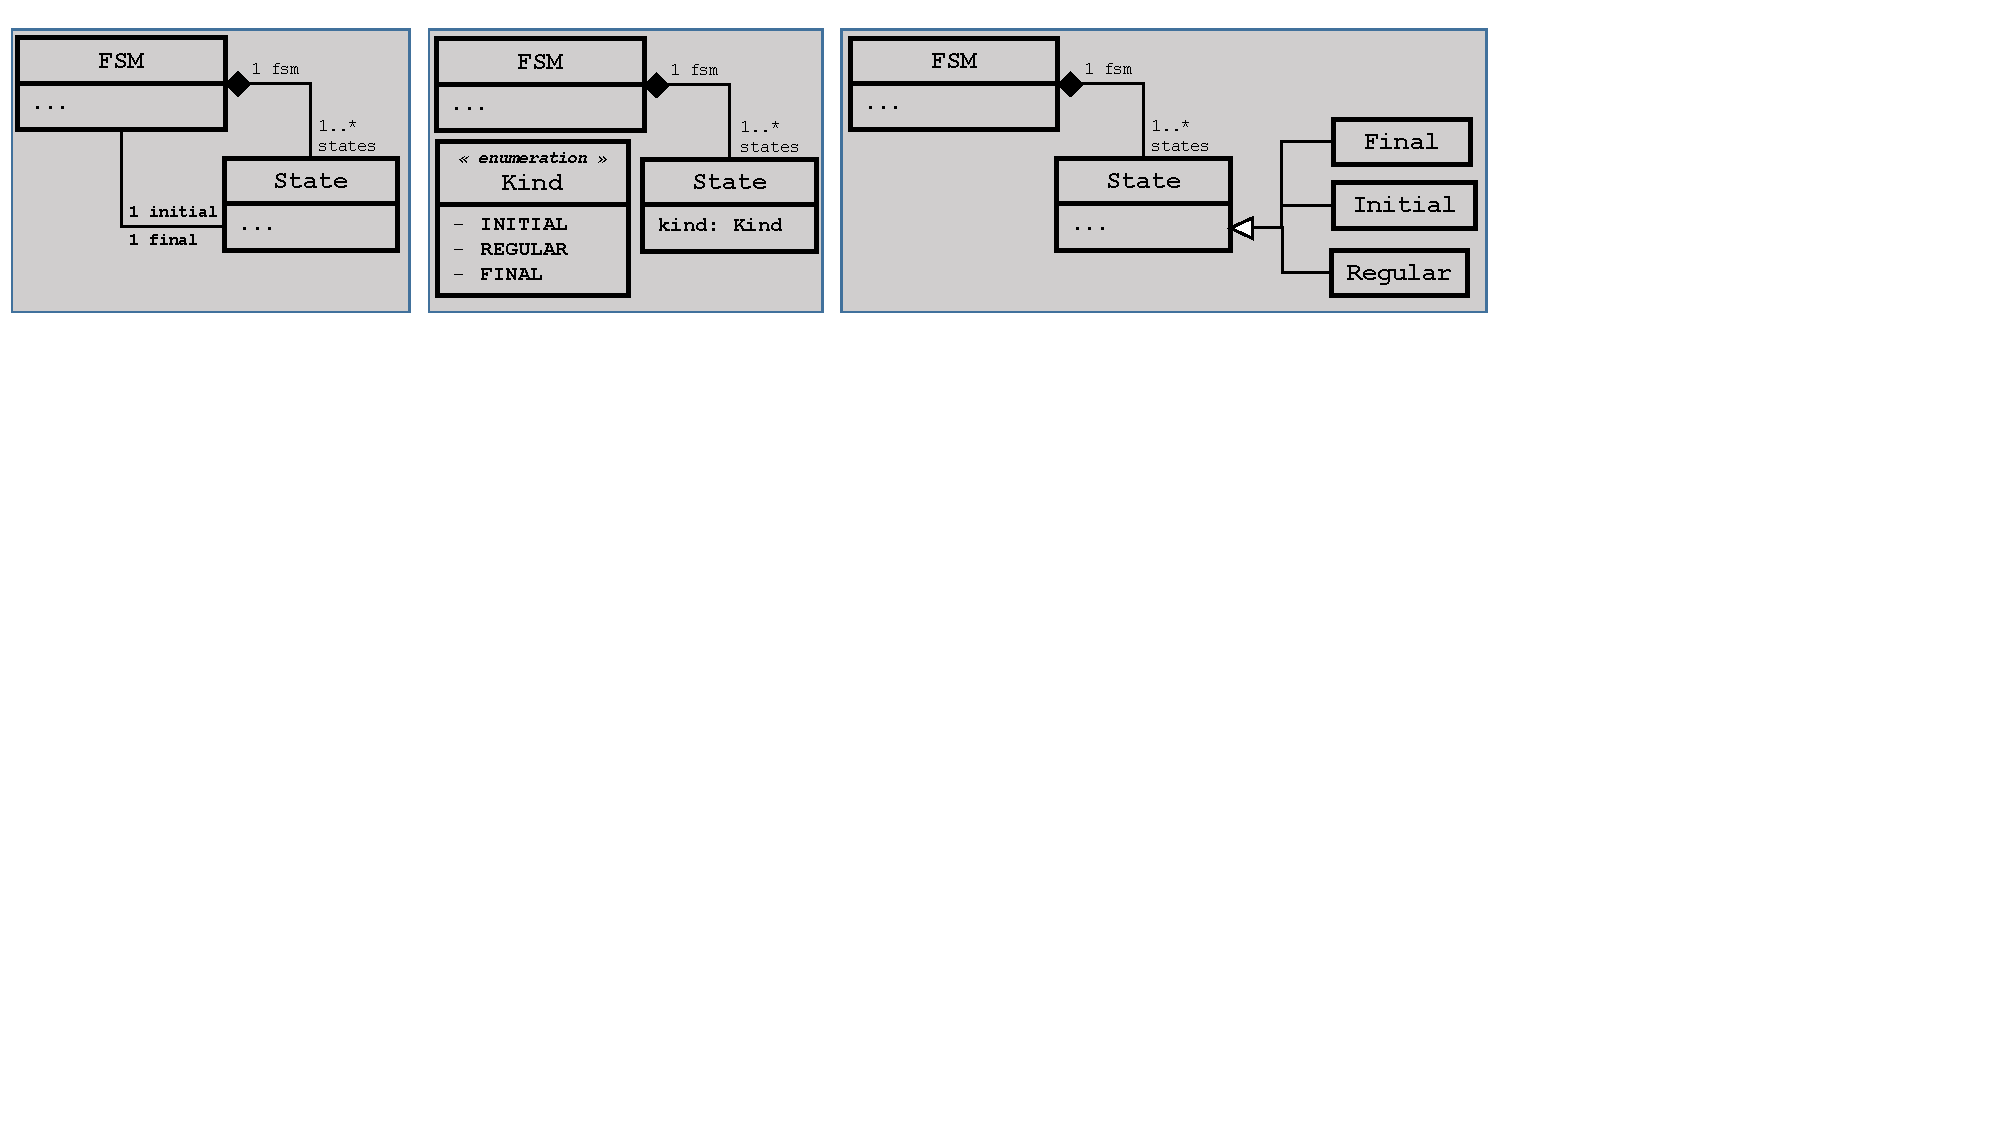
\includegraphics[width=\columnwidth,clip, trim=0cm 13.8cm 8.3cm 0.2cm]{FSM-Initial}%
   \caption{Modelling a \textsf{State} in \textsf{FSM}: with explicit references
   \texttt{initial} and \texttt{final} (left); with a distinguishing property 
   \texttt{kind} (middle); and with inheritance (right).}%
   \label{fig:FSM-Initial}%
   \Description[Different ways of modelling \textsf{FSM}'s \textsf{State}s.]{%
   A \textsf{State} is modelled with explicit references, with a distinguishing 
   property in \textsf{State} specifying, with an enumeration, the different 
   \textsf{kind}s, and with inheritance.}
\end{figure}

\begin{description}
   \item[CS.1. Providing \emph{simple} visualisation of data struc\-tures.]
   Pro\-vi\-ding configurable representations for common data structures such as
   (multi-column) tables, graphs, sets and lists present the benefit of rapidly
   presenting information from a model. This ability should rely on queries to
   identify, and eventually modify, the elements of the model used for ``populating''
   such structures. 

	\item[CS.2. Providing \emph{complex} rendering patterns.]
   Consider the (partial) meta\-models in \autoref{fig:FSM-Initial} that
   specify the \emph{initial} \textsf{State} in four different ways: by referencing
   to the appropriate \textsf{State} among those available, by characterising each \textsf{State} with
   a property \textsf{kind}, or by using type inheritance. Many tools would only
   support the latter, because they essentially only allow to 
   associate various icons to classes. This approach is too simplistic and forces
   metamodel designers to tweak their metamodels towards MA, introducing yet another
   metamodel specialisation (as it is already the case for model editing and
   model analysis, among others). Complex rendering patterns should allow to freely
   associate visual counterparts to various combinations and values of metamodel
   elements.
   
   \item[CS.3. Integrating ``insideness'' \emph{natively}] We call \emph{insideness}
   the visual equivalent of \emph{containment} in metamodelling, i.e. the ability
   to uniquely put elements \emph{inside} inside a container so that elements 
   inside disappear along with the container's removal. This feature presents two
   advantages. First, it would allow to natively handle common situations like 
   including text inside a shape (e.g. displaying a \textsf{State}'s name within
   the circle for an \textsf{FSM}) and then treat them in an universal manner. 
   Second, if the feature is customisable, it would enforce a natural semantics
   graphically with an expected behaviour. 
   
   \item[CS.4. Providing ``snapping'' capabilities] Snapping helps precise\-ly arrange
   graphical elements by ``gluing'' them to a specific target, e.g. a canva's
   boundary, a grid, or points on objects. 
      
   \item[CS.6. Supporting animations natively.] Having at disposal a \DSL
   for defining CSs brings the ability to \emph{visually} render metamodels, but
   does not guarantee the ability to perform animation. For that, the \DSL should
   natively support the fast update of visual features that compose the CS (e.g.,
   the position, size, color, type of line for an \textsf{FSM}'s 
   \textsf{Transition}).      
\end{description}



\subsection{Model Animation}
\label{sec:MA}

To answer Challenge C2, it is important to design the MA framework with
the idea of reuse at its core. One possible approach is to separate two
things: the basic blocks defining animations \emph{effects} that may be combined
into comprehensive Model Animation Units (UAs), from the way they are organised
and scheduled to build complex animations. The approach we propose is similar
to the de-/reconstruction of MTLs described by \citet{J:SyrianiVangheluwe:2013}:
the idea is to capture the most basic animation effects, and offer powerful 
mechanisms to combine them, resulting in the ability to effectively specify any
kind of animation. We quickly discuss basic effects before describing two
approaches for scheduling.



\subsubsection{UA Effects}
\label{sec:MA-Effects}

Effects may be roughly classified into four categories, depending on the features
they act on:
\begin{description}
   \item[Creation] effects bring an element into a diagram in various ways, e.g. by
   simply making it appear at the right position, or by ``zooming'' it in, i.e.
   starting from a small size until reaching its regular size, while preserving 
   the element's proportions.
   
   \item[Deletion] effects remove an elements from a diagram, e.g. by making it
   disappear, or by ``zooming'' it out. 
   
   \item[Action] effects update one, or several of the visual features of an
   element, e.g. the color, size, etc. of a text, a shape or a connector.
   
   \item[Path Motion] effects move an element along a predefined path, e.g. a
   straight or curved line, or the line represented by a connector.
\end{description}
We expect that most of the MAs would make use of a small set of basic effects. 
These effects could be organised into libraries and potentially exchanged among
MA specialists, but their reuse across different platforms may be hindered by how
effects are highly dependent on the way the graphical components of the CS are
defined.

As illustrative examples, \textsf{PM.3}, \textsf{FSM.1.2} and \textsf{PN.1} and \textsf{PN.2}
all falls into the \emph{Action} effects category, because only the graphical 
features (or values) of the score label, the \textsf{Letter} and the color of the
\textsf{Arc}(s) are modified. \autoref{fig:FSM_M} graphically illustrates,
in the middle, an possible way to realise a \emph{Path Motion} effect. Finally,
\emph{Creation} and \emph{Deletion} effects are combined to realise a complex 
animation in \textsf{FSM.2.1}, \textsf{PM.1} and \textsf{PN.3.2}. 

\subsubsection{UA Scheduling}
\label{sec:MA-Scheduling}

\begin{figure}[t]%
   \centering
   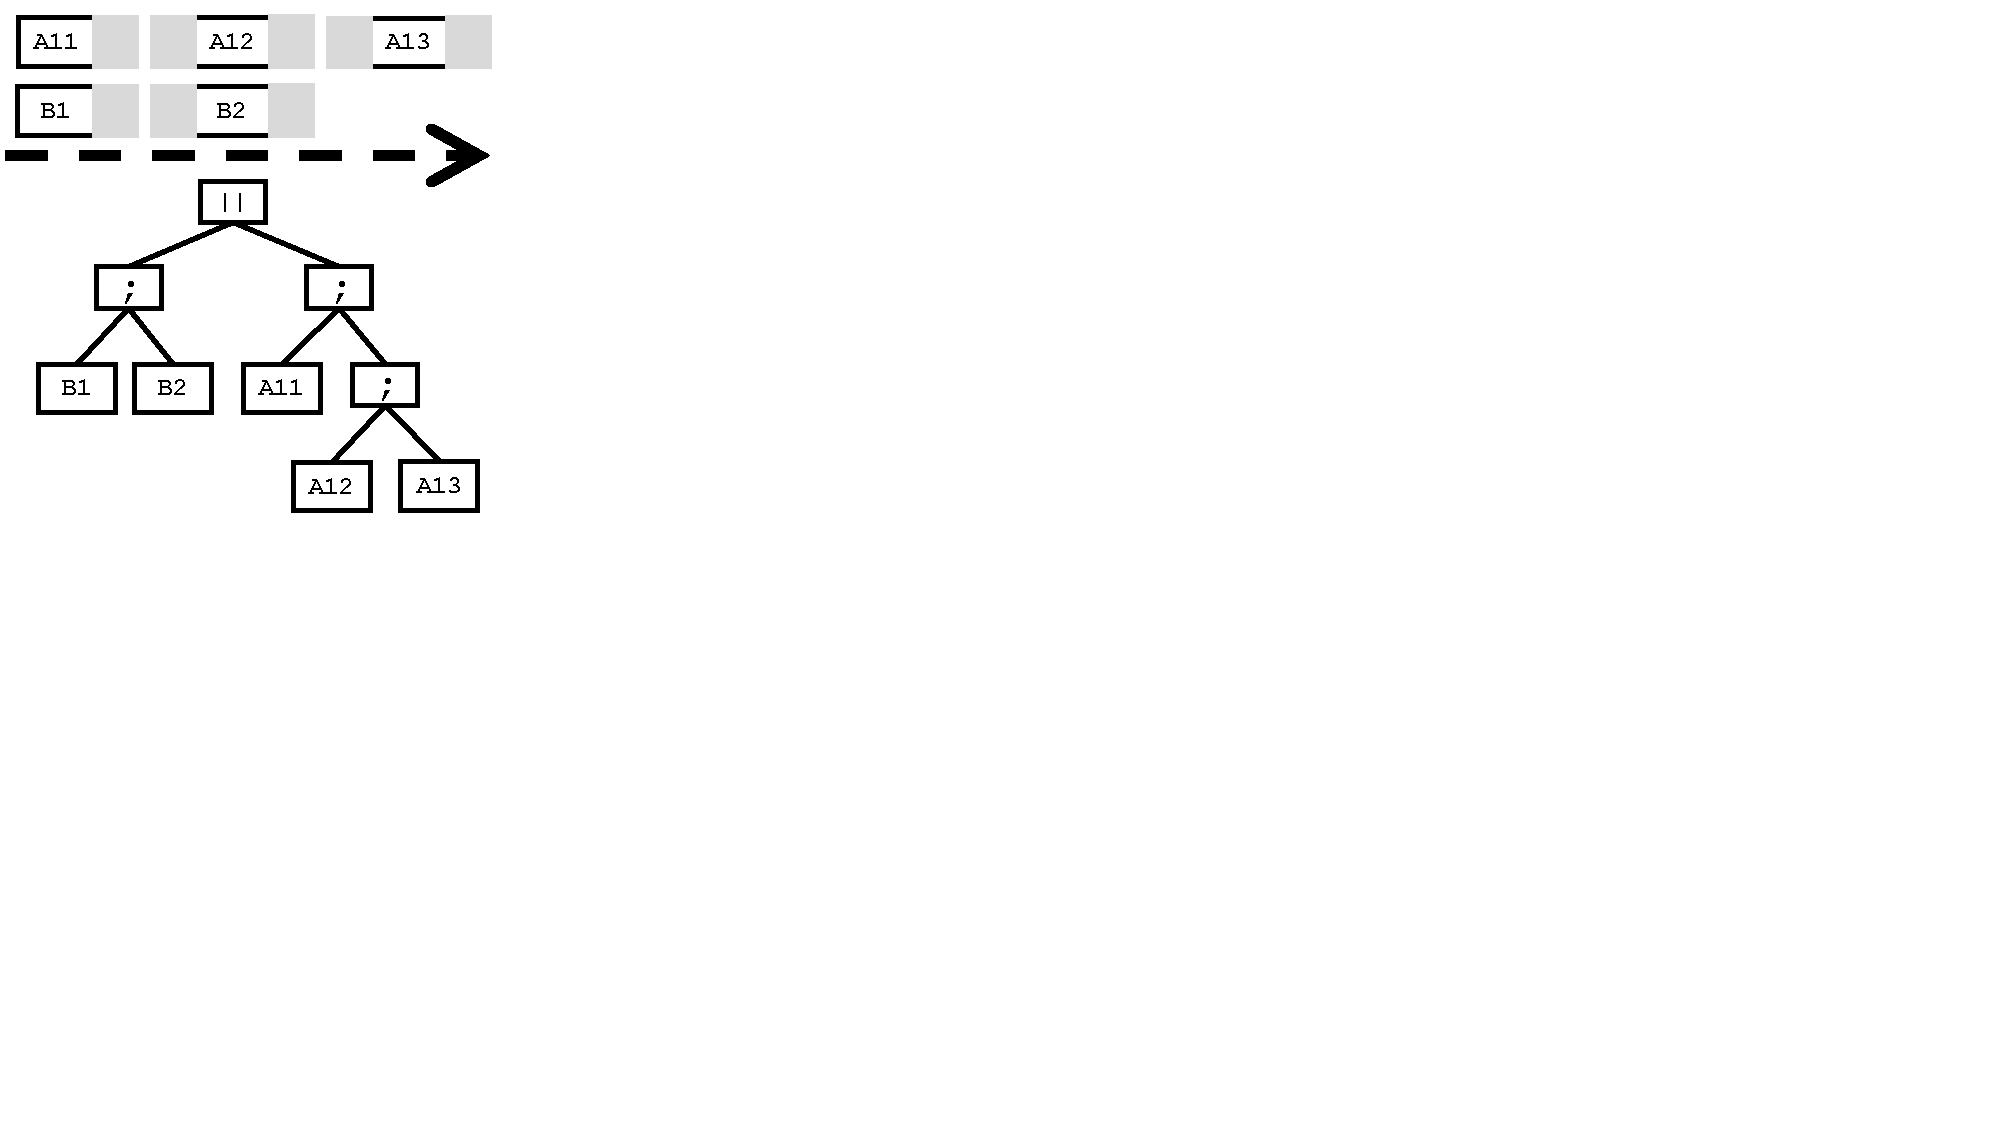
\includegraphics[width=\columnwidth,clip, trim=0cm 10cm 25cm 0.2cm]{UAScheduling}%
   \caption{On top, scheduling is realised with \emph{embedding}: each AU has 
   pre- (except the first) and post-conditions, represented as grey blocks attached 
   before and after the AU. On bottom, the same animations but with UAs organised with
   two combinators: \texttt{\textbf{||}} for parallel, and \texttt{\textbf{;}} for
   sequential combinations (the temporal details are omitted).
   }%
   \label{fig:UA-Schedule}%
\end{figure}

Although theoretically equivalent, two approaches are possible for realising
this requirement.
\begin{description}
   \item[Embedding the scheduling \emph{inside} the UAs] As suggested in 
   \autoref{fig:UA-Schedule} (left), each UA is extended with pre- and 
   post-conditions. A precondition indicates how an UA starts relatively to the 
   previous one (at the same time, after, or delayed by a given time); while a
   postcondition would define whether the UA is repeated (and how many times).
   
   \item[Define \emph{combinators outside} of UAs] Another approach, suggested
   in \autoref{fig:UA-Schedule} (right) is to provide explicit \emph{combination}
   operators (aka. \emph{combinators}) that would take as operands UAs. Combinators
   similar to the previous case may be defined: sequencers with a possible delay,
   repetitors, and parallelisation. 
\end{description}
The second approach may seem more familiar to MA designers with a programming 
background, because the combinators approach proposes constructions similar to
what is available in GPLs. However, the first approach may be more compact visually,
and familiar for MA designers accustomed to slideshow tools (the most popular and
mainstream ones being Microsoft Powerpoint, Apple Keynote and Google Slides, among
a plethora of other dedicated tools, many of which only existing online).

Note that both approaches may concurrently exist, allowing MA designers to choose
the most appropriate approach for specifying their MA. It is left as future work
to study under which conditions they may coexist (if possible at all), and to 
identify when and how each presents more benefits than the other.

\subsection{Parameterisation of Animation}
\label{sec:Param}

What we mean by \emph{parameterisation} is the ability, for an AU, to separate 
the internal animation logic so that it becomes possible to apply it consistently
to elements from different \DSLs, thus promoting reuse. Taking our \DSLs of \S 
\ref{sec:Examples}, we see that \textsf{PM.1}, \textsf{FSM.2.1} and \textsf{PN.3.1}
all involve the same animation logic (\emph{disappear} from the current location, 
followed by \emph{appear} on another location), but applied to different elements:
in \textsf{PM}, it concerns the \textsf{Persona}; in \textsf{FSM}, it concerns the
\textsf{Token}; and in \textsf{PN}, it iteratively applies to the markings.

The exact mechanism required for implementing this feature into MA is beyond this
paper's scope. However, there is essentially two ways to realise it:
\begin{description}
   \item[Using model's elements] The first one consists of explicitly referencing
   the model's elements (either objects or links). Retrieving the corresponding 
   graphical elements can be achieved through the mapping to the CS. This approach
   has the advantage of directly reusing the models, preventing MA designers from
   any extra work. However, the task may be complicated by the presence of complex
   rendering patterns that need to be computed before determining which graphical
   object the AU logic applies to.
   
   \item[Using the graphical elements] The second, and opposite approach consists
   of directly referencing the graphical elements impacted by an AU. In this case,
   the UA does not depend on the complexity of rendering patterns, but has the 
   drawback of preventing to easily retrieve which elements in the model have been
   impacted by an animation.
\end{description}

\autoref{fig:UA-Param} shows how parameters could be integrated into animations. 
Two basic animation units \textsf{APP} (making an element appear) and \textsf{DAPP}
(making an element disappear) with their respective parameters. They are then
composed into a complex unit \textsf{BLINK}, which exposes the parameters of
the previous units and adds a new one for controlling the blinking delay.

\begin{figure}[t]%
   \centering
   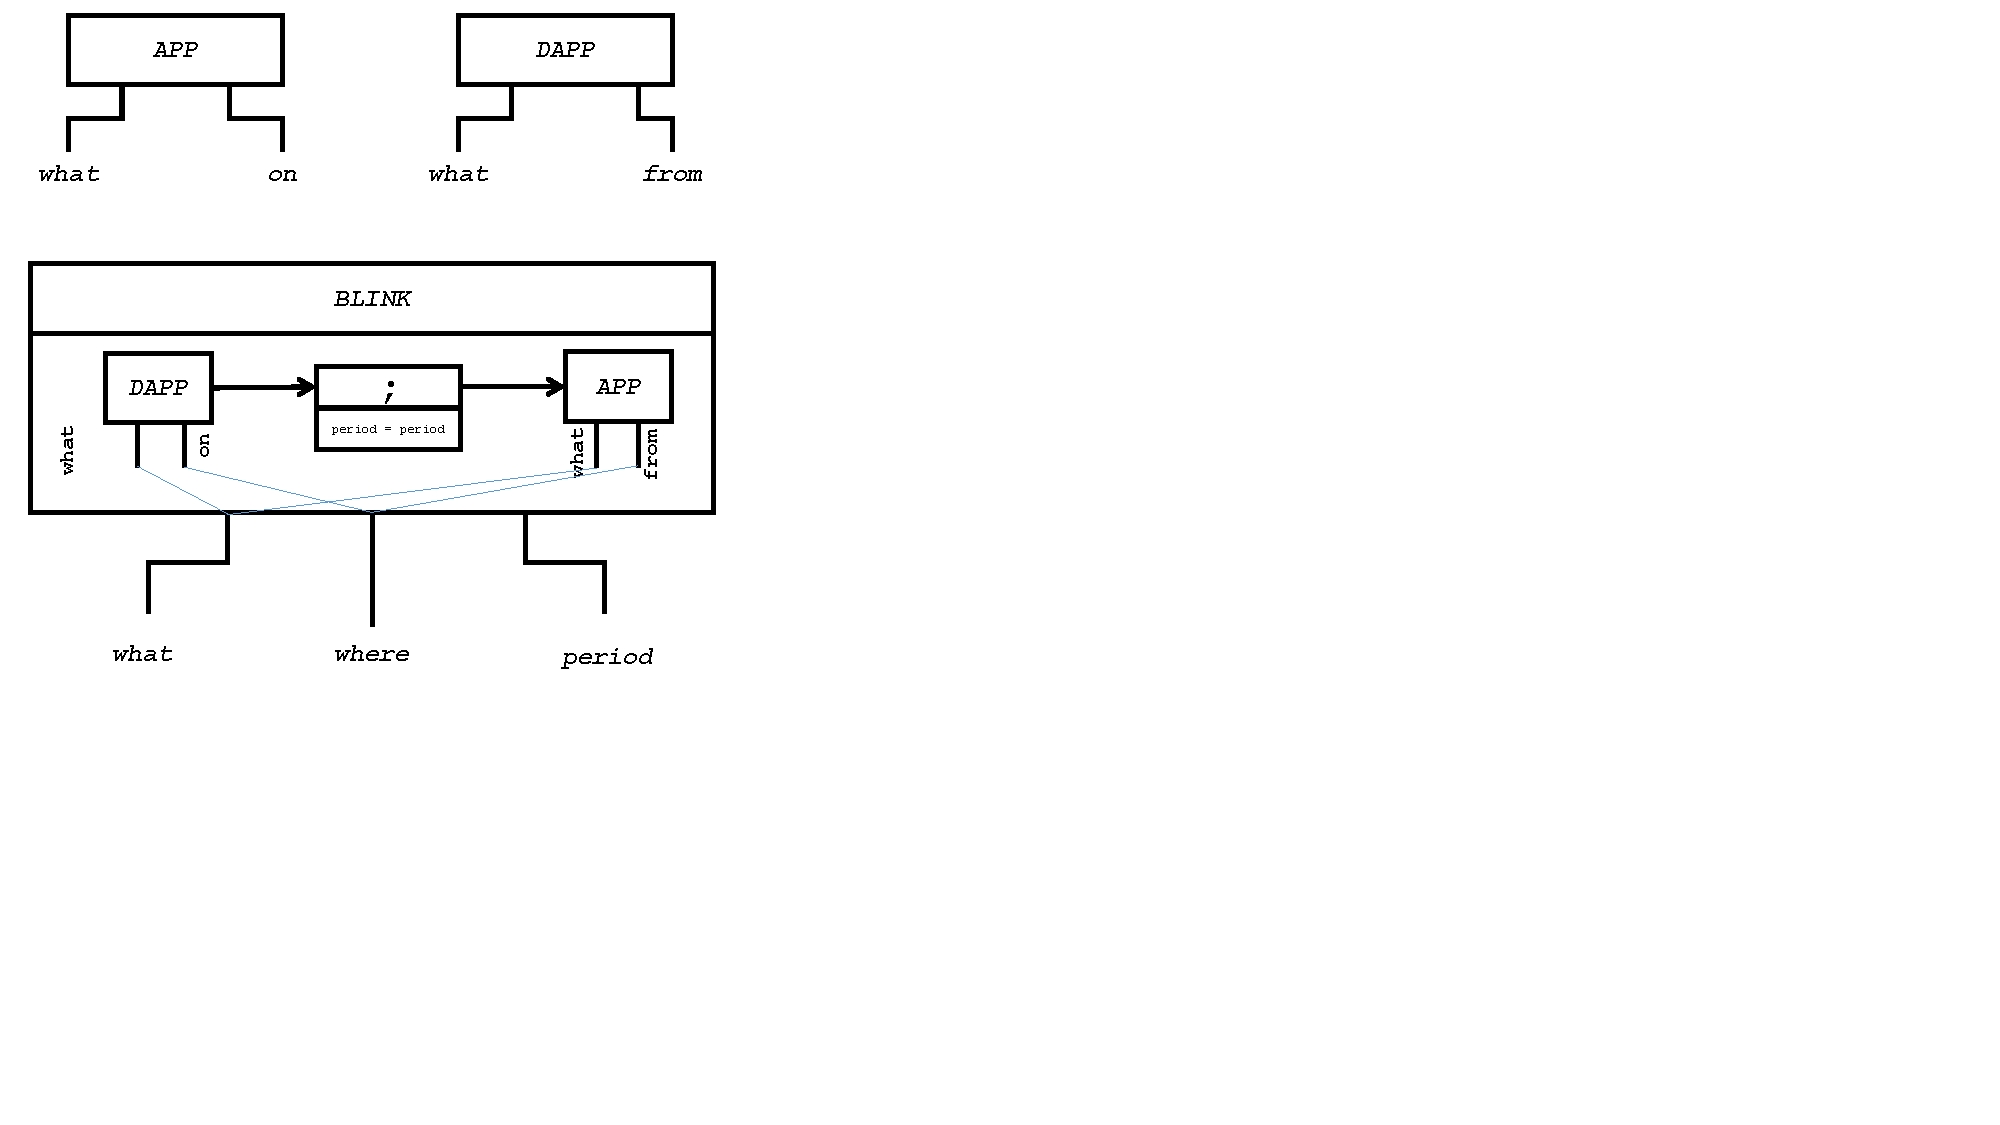
\includegraphics[width=\columnwidth,clip, trim=0cm 7.5cm 21cm 0cm]{UAs}%
   \caption{Two basic AUs: \textsf{APP} make the object \textsf{what} \emph{appear}
   \textsf{on} a location; and \textsf{DAPP} make one \emph{disappear}. Then,
   \textsf{BLINK} combines both to make an object \emph{blink} at a defined
   \textsf{period}.
   }%
   \label{fig:UA-Param}%
\end{figure}
\subsection{Linking AUs and TUs}
\label{sec:AUTU}

We already assumed that AUs are ``mapped'' to specific TUs of the MT defining
a \DSL's execution semantics. Depending on the underlying MTL, this mapping may
be given in two ways: by annotating the TUs with the information (typically,
an AU name that allows to retrieve an associated MA specification); conversely,
by annotating the AUs with the TUs they refer to; or using an explicit map
defined outside both the MT and MA specifications. The first approach has already
been successfully used for mapping TUs with debugging steps in \cite{bousse2018omniscient}.

Relating AUs with TUs provides a simple advantage: since the MT already captures
the internal logic and scheduling between TUs, no need to reproduce them for the
AUs. However, this imposes that the execution engine is instrumented for enabling
simple communication with the MA engine. As a first starting step, adopting the 
generic interface for debugging proposed by \citet{bousse2018omniscient} provides
what is necessary: it indicates the MA engine that a simulation has started and
stopped, and that a TU has started (together with appropriate parameters) and 
stopped.

 
\section{Proposal}
\label{sec:Proposal}

This Section wraps up the previous considerations by making a partial proposal
for the missing elements, so that it becomes possible to demonstrate that our vision
works. We demonstrate that it becomes possible to specify MAs independently of the
MT specifying a \DSL's execution semantics; that several MAs may be linked to
the same MT for animating a model according to the viewer's preferences; and finally
that MAs may be reused accross \DSLs.

%We start by specifying a prototype metamodel \textsf{CS} for specifying concrete
%syntaxes explicitly. We then define 

\subsection{\textsf{VCS}: The Visual Concrete Syntax \DSL}
\label{sec:Proposal-VCS}

\autoref{fig:VCS} shows the metamodel of a \textsf{VCS}, a simplified \DSL designed
for the specification of Visual Concrete Syntaxes. It consists of a \textsf{Canva}
of variable size where graphical elments (\textsf{GElement}) may be geometrically
placed. A \textsf{GElement} follows the Composite Pattern \citep{B:Gamma-etAl:1995}:
\textsf{Shape}s may be \emph{composed}, i.e. the \textsf{containee} is displayed
\emph{inside} the \textsf{container} with specific alignment features. 

A \textsf{Shape} is either a \textsf{Table}, a \textsf{TextBox}, or a 
\textsf{Geometric} element, which is either a \textsf{Form} or a 
\textsf{Connector}. Each \textsf{Shape} is inscribed into a bouding box with specific 
dimensions that helps precisely positioning it on the \textsf{Canva}, and also
defines specific features: for example, a Rectangle may define the thickness of its
external box, and an Arrow may define different types and sizes for their heads.
A \textsf{Shape} may also define a \textsf{Style} that can be \textsf{name}d and
reused for other \textsf{Shape}s, to specify various features such as the background
or line colour, the line transparency, etc.

This metamodel captures insideness with \textsf{Composer}, and may easily be extended
with additional \textsf{Shape}s that only need to be encapsulated in a box (thus,
giving value to the attributes \textsf{length} and \textsf{height} in \textsf{Shape}).


\begin{figure}[t]%
   \centering
   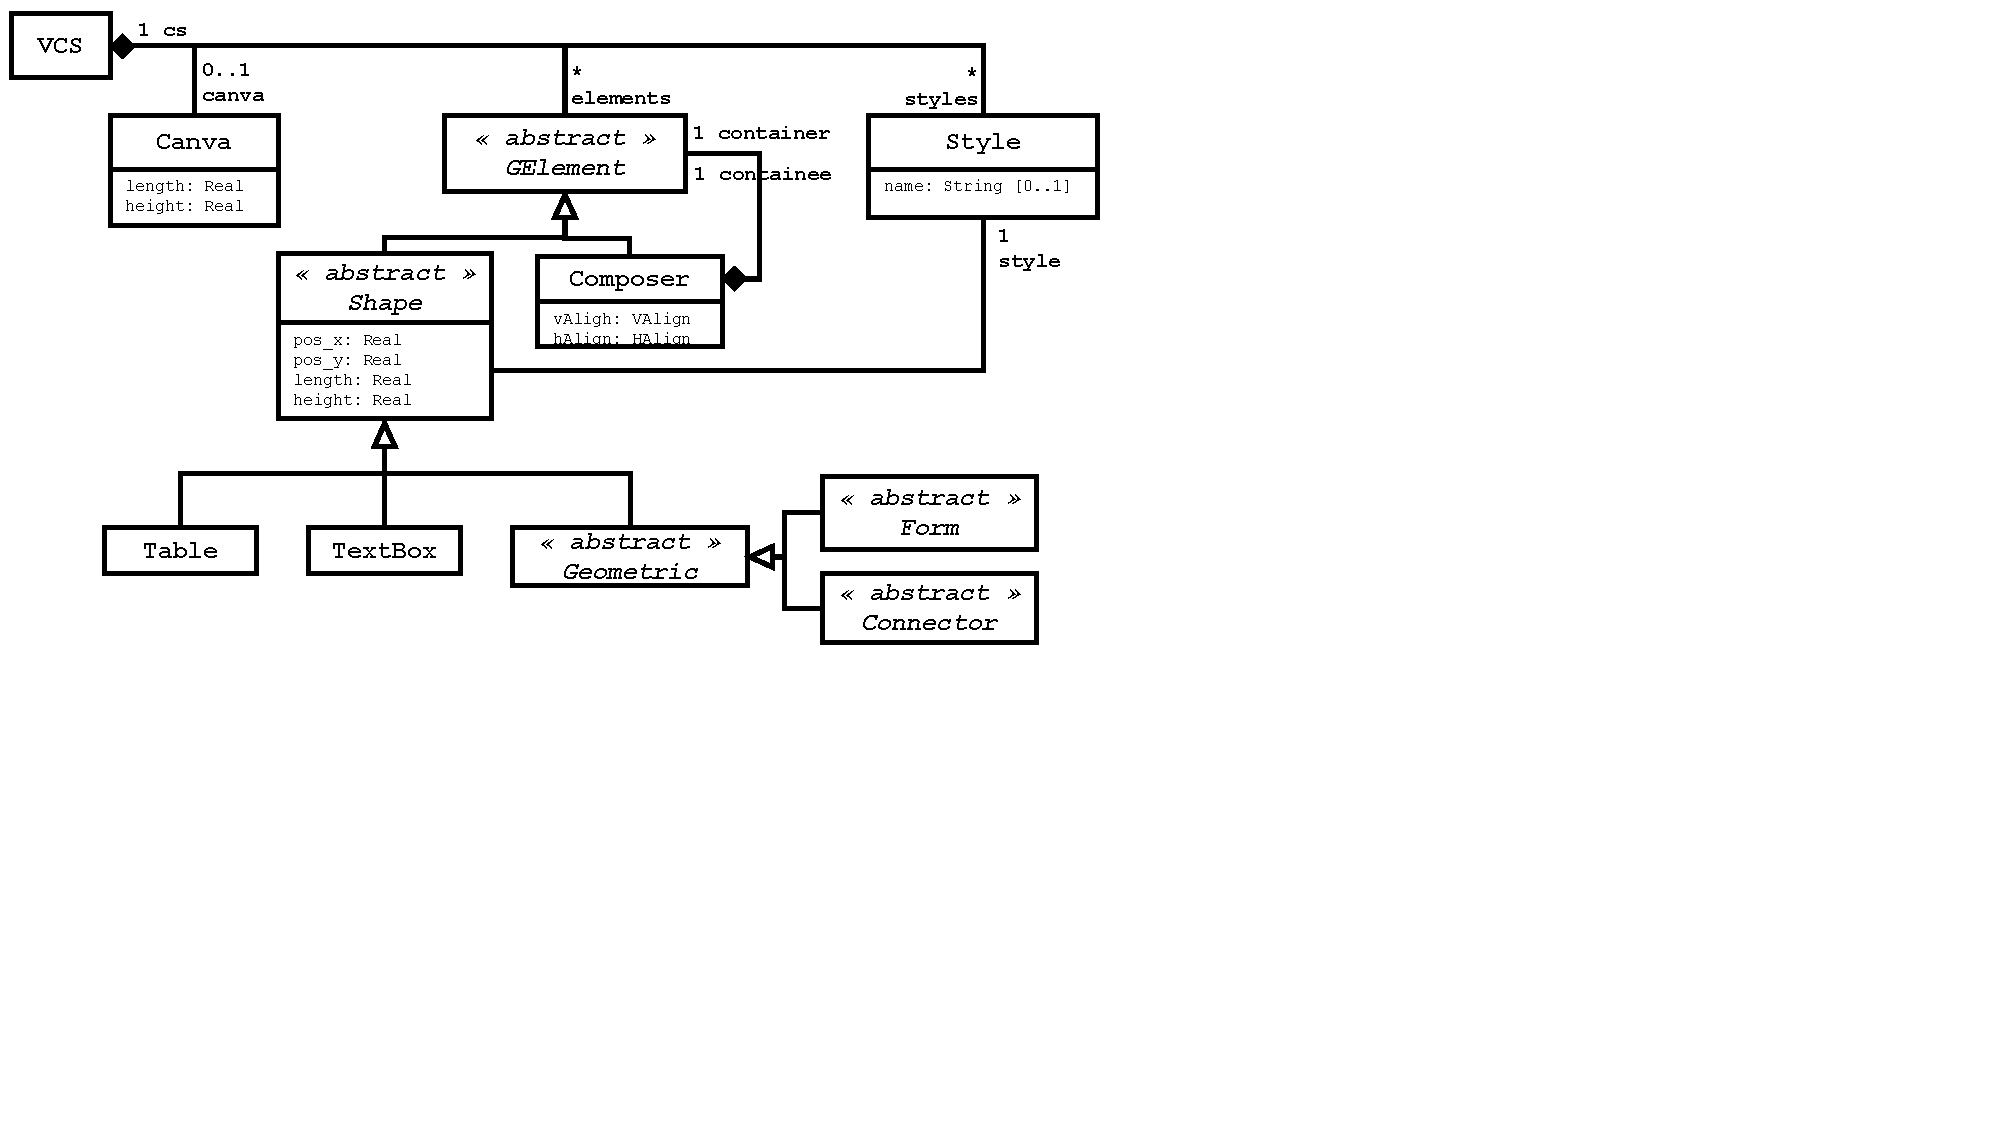
\includegraphics[width=\columnwidth,clip, trim=0cm 9cm 15cm 0.2cm]{VCS}%
   \caption{\textsf{VCS}: A simplified \DSL for specifying \emph{V}isual \emph{C}oncrete \emph{S}yntaxes}%
   \label{fig:VCS}%
\end{figure}


\subsection{Revisiting the \textsf{FSM}}
\label{sec:Proposal-FSM-CS}

We now informally define a mapping from the \DSL specifying the abstract syntax 
of the \FSM \DSL, as presented in \autoref{fig:FSM_MM}, with the elements of 
\textsf{VCS}. 

The \textsf{FSM} itself is simply mapped to the general \textsf{Canva}, but we put
a \textsf{TextBox} on the top left that will display the value of \textsf{FSM::name}.
A \textsf{State} will be represented by an \textsf{Ellipse} with equal \textsf{length}
and \textsf{height} (thus forming a circle) drawn in black. A final \textsf{State}
is simply the composite of two \textsf{Ellipse}s vertically and horizontally centered,
whose dimensions only differ by a specific delta. For the purpose of simplification,
we will represent initial states with a similar \textsf{Ellipse} using a dotted line.
A \textsf{Transition} will be represented by a \textsf{Curved} \textsf{Connector}
using a black, plain line, with the same thickness as the \textsf{Ellipse}s, and
with an \textsf{Arrow} of the biggest size on the end part. 

Following the traditional approach in \MDE, this mapping should generate a so-called
\emph{palette} that allows modellers to create their models. From this simple example,
we see that such a definition should introduce flexibility for the modeller. 
For example, the \textsf{Transition} may require different types of \textsf{Connector}s
depending on the model's complexity.

\section{Related Work}
\label{sec:RW}

MA is integrated in various tools that differ in the way the underlying MT is specified.
GeMoC \citep{combemale2016tool} relies on Obeo Sirius for performing the MA of 
\DSLs whose behavioural semantics is expressed in the Kermeta3 or Xtend languages.
AtoMPM \cite{Syriani-Vangheluwe-etAl:2013} supports the specification of MTs
based on Graph Rewriting, and provides support for specifying a concrete syntax
for a \DSL that allows to both express MT rules using the concrete syntax (by
relying on the RAMification process \cite{Kuehne-Mezei-etAl:2009}), and to 
debug and animate a model. Earlier, \citet{Sadilek-Wachsmuth:2008} proposed eProvide,
an Eclipse-based tool that, given the specification of the ``runtime state''
and a visual concrete syntax, automatically generates a visual interpreter and a 
visual debugger for executing a \DSL. ProB \cite{leuschel2008prob} is a model-checker
and visualiser for B specifications. It has been used in Meeduse \cite{idani2020meeduse},
an visualiser and analyser for \DSLs whose semantics is specified with B, and allows
step-by-step execution and animation.

Many frameworks that allow modellers to express \DSL semantics using formalisms
that natively have a visual representation provide animators for free. Such examples
include Finite-State Machines \cite{Das2016SupportingTM,Goldsby-etAl:2006,Bandener-etAl:2010}
and Petri Nets \cite{mosteller2019integrated,Palanque-etAl:2009,Wimmer-etAl:2009}.
Although the animation facilities are greatly simplified, this approach does
not support domain-specific visual concrete syntax: the animation is realised 
directly on the underlying formalism, preventing flexibility and adaptivity.

MA can also be performed \emph{offline}, i.e. aside from the MT execution itself.
In this case, information about one, or several, execution(s) of a \DSL need to
be collected beforehand, and ``replayed'' by the MA engine in order to visually
represent the execution(s). Generally, this information is collected in the form
of execution traces \cite{J:Hojaji-Mayerhofer-etAl:2019} that represent the dynamic
state of the \DSL along the execution. Although this approach does not strictly 
fit our definition of MA, it is interesting because it highlights the importance
of properly identifying what a dynamic state is, and the possibility to reuse
the MA engine for different purposes. Several contributions follow this approach
\cite{J:Hegedues-Rath-Varro:2012,Guin-Syriani:2013,idani2021formal}, with different
MT languages.

Modelling \& Simulation \cite{B:Birta-Arbez:2019} is a closely related research 
area addressing large Cyber-Physical Systems, where the behaviour is usually expressed
through formalisms that include real-time, and sometimes continuous space variables,
based on physical phenomena that require complex behaviour captured through, among
others, differential equations. Although the behaviour of such systems is clearly
out of scope of \MDE, the tools supporting these specifications often propose 
\emph{visual} simulation (e.g. Ansys Simplorer, 20-sim, MapleSoft MapleSim, etc.)
They do not strictly compare to our proposal, but many ideas and concerns from the
literature of this research area may help designing better animators. 

Debugging, and in particular omniscient debugging 
\citep{bousse2018omniscient,J:Corley-Eddy-Syriani-Grey:2016,J:VanMierlo-Vangheluwe-etAl:2020},
is a topic closely related to MA, as it shares some of the underlying mechanisms,
such as the definition of a TU considered as a candidate \emph{step} for debugging,
and the protocols used to communicate between the transformation engine and the debugger.
\citet{bousse2018omniscient} introduce two interesting notions that we have reused
in our vision. First, \emph{annotation steps} indicate which parts of a MT (our TUs) may safely
be interrupted for inspection during debugging. Second, an \emph{interruption pattern}
(based on the more well-known Observer pattern \cite{B:Gamma-etAl:1995}) specifies
a minimal interface for external services, typically the debugger, to interrupt
the execution engine at the beginning and end of the execution, and at key moments
when annotation steps are reached. \citet{J:VanMierlo-Vangheluwe-etAl:2020} provide
a reusable architecture and an explicitly modelled workflow to support debuggers
construction. An interesting feature is the ability to rely on a visual representation
of the models being simulating, thus providing a form of animation.
\section{Conclusion}
\label{sec:Conclusion}

Model Animation (MA) is a popular approach for providing visual clues for model transformation
designers, as well as modellers, that should contribute to help them better 
understand, and ultimately correct, their models and the associated transformations.
This is because MA is closely related to the execution of \DSLs: MA visually represent
meaningful steps of the model transformations. 

As a first step towards a systematic approach for MA engineering, we have 
identified in this paper three important challenges. 
First, designing concrete syntaxes for \DSLs is not trivial, and this should support
complex patterns in order to explicitly express the so-called \emph{mapping}, i.e.
the rendering transformation between the \DSL metamodel capturing its abstract syntax,
into the metamodel describing graphical components. This latter metamodel is a \DSL
on its own right, and should natively support animation, i.e. the timely and 
effective change in the graphical components's features (e.g. size, color, thickness,
and general topology of elements such as tables, rectangles, etc.)

Second, we plea for a compositional approach for defining complex MA, because relying
on basic constructions that are combined to form complex animations promotes flexibility
and reuse. The flexibility of a dedicated MA \DSL should open the ability to 
parameterise MA definitions, so that the internal logic of the MA becomes independent
from the graphical elements it is applied to. Just like methods may be used in 
different context captured by the method's parameters, an MA should have parameters
to explicitly designate which elements are taken into account, and how. The reuse
of an MA \DSL should allow to apply the same MA, which uses the same logic underneath,
across multiple \DSLs that have the same animation logic. We have shown on simple
examples that both properties, flexibility and reuse, are effectively found in
very simple \DSLs, and should appear in bigger ones as well. In turn, these properties
should promote the exchange and reuse of well-defined libraries of animations, thus
facilitating the specification of future MAs.

Third, in order to not reinvent the logic behind the Model Transformation capturing
a \DSL's behavioural semantics, an MA should be linked to appropriate Transformations
Units (TUs) that would drive the MAs. This way, it becomes possible to extensively
reuse the Model Transformation specification as well as its scheduling logic, and
only trigger appropriate MA pieces (that we called Animation Units) that would
visually reflect what a TU is achieving. 

We are aware that MA is a novel field, thus lacks maturity both in terms of methodologies
and tooling. However, by identifying these challenges, by providing some leads on
how it could be possible to at least partially meet them, while still applying
the \MDE approach (and in particular, defining carefully designed \DSLs for each
of the above tasks), we hope to pave the way towards a new and systematic approach
for MA. This, in turn, should create a new role for \MDE: MA designer, alongside
the usual role of modeller, \DSL builder and MT specialist. As the field is still
in its infancy, we are planning to approach the literature more systematically,
in order to uncover what the current practice is, how it may be possible to 
formalise the \DSLs dedicated to the tasks we identified, and identify the various
features of animators as a tool in the collection of tools for \MDE workbenches.
\newpage
\balance
\bibliographystyle{plainnat}
\bibliography{./MLE}
\end{document}
